\documentclass[11pt,a4paper]{article}
% Build: latexmk -pdf documentation.tex, then copy documentation.pdf to docs/.
% Data figures (data/*.pdf): python scripts/doc_figures.py data/demo docs/documentation/data
% Demo figures (../figures/*.png): phasewall demo data/demo, copied from data/demo/walls/.

\usepackage[T1]{fontenc}
\usepackage{lmodern}
\usepackage[margin=2.4cm]{geometry}
\usepackage{microtype}
\usepackage{amsmath,amssymb,mathtools,bm}
\usepackage{booktabs}
\usepackage{array}
\usepackage{enumitem}
\usepackage{xcolor}
\usepackage{graphicx}
\usepackage{tikz}
\usetikzlibrary{positioning,arrows.meta,calc,decorations.pathreplacing,fit,backgrounds}
\usepackage{float}
\usepackage[most]{tcolorbox}
\usepackage[colorlinks=true,linkcolor=blue!50!black,urlcolor=blue!50!black,citecolor=blue!50!black]{hyperref}

\setlength{\parindent}{0pt}
\setlength{\parskip}{0.5em}
\setcounter{tocdepth}{2}

% Two kinds of boxes, printable (white background): mathematics and physics parallel (blue,
% thick left bar), code (orange, dashed).
\tcbset{pwbox/.style={enhanced, breakable, colback=white, coltitle=black,
  fonttitle=\bfseries\small, left=6pt, right=6pt, top=9pt, bottom=6pt,
  attach boxed title to top left={xshift=5mm, yshift*=-\tcboxedtitleheight/2},
  boxed title style={colback=white, colframe=white, boxrule=0pt, sharp corners,
    left=2pt, right=2pt, top=0pt, bottom=0pt},
  before upper={\setlength{\parskip}{0.5em}}}}
\newtcolorbox{tech}{pwbox, title={Mathematics and physics parallel}, sharp corners,
  colframe=blue!50!black, coltitle=blue!50!black, boxrule=0.5pt, borderline west={2.5pt}{0pt}{blue!50!black}}
\newtcolorbox{codebox}{pwbox, title={Code}, sharp corners, frame hidden, coltitle=orange!55!black,
  borderline={0.7pt}{0pt}{orange!55!black, dashed}, before upper={\setlength{\parskip}{0.4em}\raggedright}}

\newcommand{\repo}{https://github.com/Lu-Dumoulin/PhaseWall}
\newcommand{\srcref}[1]{\href{\repo/blob/main/#1}{\texttt{\detokenize{#1}}}}
\newcommand{\code}[1]{\texttt{\detokenize{#1}}}
\newcommand{\avg}[1]{\langle #1 \rangle}
\newcommand{\pw}{\texttt{phasewall}}
\DeclareMathOperator{\std}{std}
\DeclareMathOperator{\cut}{cut}
\DeclareMathOperator{\vol}{vol}
\DeclareMathOperator{\med}{med}
% Shared colours and styles of the schematics (input once in the preamble).
% The phase colours are those of phasewall.report, so schematics and data figures agree.
\definecolor{cP0}{HTML}{2A78D6}    % phase 0 (stripes in the demo)
\definecolor{cP1}{HTML}{EB6834}    % phase 1 (hexagons)
\definecolor{cP2}{HTML}{1BAF7A}    % phase 2 (uniform)
\definecolor{cInk}{HTML}{0B0B0B}
\definecolor{cInk2}{HTML}{52514E}
\definecolor{cGrid}{HTML}{C9C8C3}
\definecolor{cNeg}{HTML}{184F95}   % negative values (field maps)
\definecolor{cPos}{HTML}{B23A39}   % positive values
\definecolor{cAcc}{HTML}{D55E00}   % accent: thresholds, the wall

\tikzset{
  fig/.style={font=\small, >={Stealth}},
  lab/.style={font=\footnotesize\bfseries, align=center},
  note/.style={font=\footnotesize, align=center},
  small/.style={font=\scriptsize, align=center},
  blk/.style={draw, rounded corners, align=center, font=\footnotesize, inner sep=4pt, fill=black!3},
  dot/.style={circle, fill=#1, inner sep=0pt, minimum size=4pt},
  wall/.style={cAcc, line width=1.4pt},
}


\title{\textbf{phasewall: method, mathematics and tests}\\[0.3em]
\large Phases of simulated systems from the walls between them in parameter space}
\author{Ludovic Dumoulin}
\date{Version 0.1, 17 November 2026}

\begin{document}
\maketitle

\begin{abstract}
\pw{} takes an ensemble of simulations already run on a grid of parameters and estimates the
phases of the scanned range, without labels and without being told how many phases there are.
Every snapshot is described by generic numbers; neighbouring parameter points are compared; a
wall is placed where the description changes more than it varies within one point. This
document explains each step twice: with its mathematics and a parallel from physics (blue
boxes), and with the code that implements and tests it (orange boxes). The method is checked on the Swift-Hohenberg equation, whose three states are
known; all numbers and data figures come from that demo and from synthetic tests, made by
\srcref{scripts/doc_figures.py}.
\end{abstract}

{\setlength{\parskip}{0pt}\tableofcontents}
\newpage

%======================================================================
\section{Overview}\label{sec:overview}
%======================================================================

\begin{figure}[H]
\centering
% Overview: from runs on a parameter grid to phases.
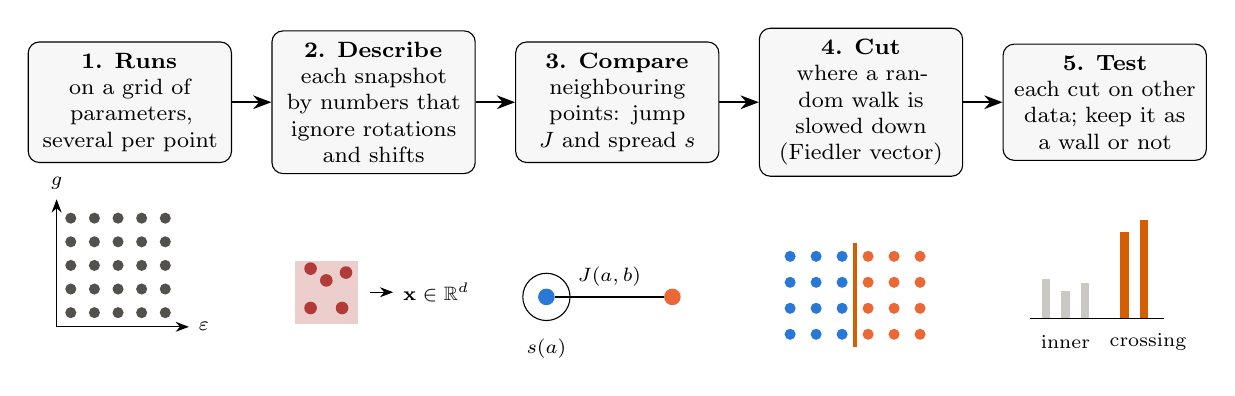
\begin{tikzpicture}[fig, node distance=0.5cm]
\node[blk, text width=2.3cm] (runs) {\textbf{1. Runs}\\ on a grid of parameters, several per point};
\node[blk, text width=2.3cm, right=of runs] (desc) {\textbf{2. Describe}\\ each snapshot by numbers that ignore rotations and shifts};
\node[blk, text width=2.3cm, right=of desc] (jump) {\textbf{3. Compare}\\ neighbouring points: jump $J$ and spread $s$};
\node[blk, text width=2.3cm, right=of jump] (cut) {\textbf{4. Cut}\\ where a random walk is slowed down (Fiedler vector)};
\node[blk, text width=2.3cm, right=of cut] (test) {\textbf{5. Test}\\ each cut on other data; keep it as a wall or not};
\foreach \a/\b in {runs/desc, desc/jump, jump/cut, cut/test} \draw[->, thick] (\a) -- (\b);
% small pictures under each box
\begin{scope}[shift={($(runs.south)+(-0.75,-1.9)$)}, scale=0.3]
  \foreach \i in {0,...,4} \foreach \j in {0,...,4} \node[dot=cInk2] at (\i,\j) {};
  \draw[->] (-0.6,-0.6) -- (5,-0.6) node[right, small] {$\varepsilon$};
  \draw[->] (-0.6,-0.6) -- (-0.6,4.8) node[above, small] {$g$};
\end{scope}
\begin{scope}[shift={($(desc.south)+(-1.0,-1.9)$)}]
  \fill[cPos!25] (0,0) rectangle (0.8,0.8);
  \foreach \x/\y in {0.2/0.2, 0.6/0.2, 0.4/0.55, 0.2/0.7, 0.65/0.65} \fill[cPos] (\x,\y) circle (0.08);
  \draw[->] (0.95,0.4) -- (1.25,0.4);
  \node[small, anchor=west] at (1.25,0.4) {$\mathbf{x}\in\mathbb{R}^{d}$};
\end{scope}
\begin{scope}[shift={($(jump.south)+(-0.9,-1.7)$)}]
  \node[dot=cP0, minimum size=6pt] (a) at (0,0) {};
  \node[dot=cP1, minimum size=6pt] (b) at (1.6,0) {};
  \draw[thick] (a) -- node[above, small] {$J(a,b)$} (b);
  \draw (a) circle (0.3); \node[small, below=0.3 of a] {$s(a)$};
\end{scope}
\begin{scope}[shift={($(cut.south)+(-0.9,-2.0)$)}, scale=0.33]
  \foreach \i in {0,...,2} \foreach \j in {0,...,3} \node[dot=cP0] at (\i,\j) {};
  \foreach \i in {3,...,5} \foreach \j in {0,...,3} \node[dot=cP1] at (\i,\j) {};
  \draw[wall] (2.5,-0.5) -- (2.5,3.5);
\end{scope}
\begin{scope}[shift={($(test.south)+(-0.75,-2.0)$)}]
  \draw[cGrid, line width=3pt] (0,0) -- (0,0.5); \draw[cGrid, line width=3pt] (0.25,0) -- (0.25,0.35);
  \draw[cGrid, line width=3pt] (0.5,0) -- (0.5,0.45);
  \draw[cAcc, line width=3pt] (1.0,0) -- (1.0,1.1); \draw[cAcc, line width=3pt] (1.25,0) -- (1.25,1.25);
  \draw (-0.2,0) -- (1.5,0);
  \node[small] at (0.25,-0.3) {inner}; \node[small] at (1.3,-0.3) {crossing};
\end{scope}
\end{tikzpicture}

\caption{The five steps of \pw{}. Steps 1 and 2 read the data; steps 3 to 5 work only on the
table of descriptors, so any other description (for example the output of a neural network)
can be used instead.}\label{fig:pipeline}
\end{figure}

\begin{tech}
A phase transition is a place in parameter space where a macroscopic property changes
abruptly: in an infinite system, a non-analyticity of the free energy. A simulated scan
only samples a finite system at discrete points, so the question becomes statistical:
between which neighbouring points does the \emph{distribution} of the description change
more than a smooth variation and sampling noise can explain? \pw{} (Fig.~\ref{fig:pipeline}) treats the scan as a graph
(nodes: parameter points; links: neighbours) and looks for cuts of this graph, in the same
spirit as domain walls are located in a magnet: the order parameter is here the whole
distribution of descriptors at a point, and ``space'' is the parameter grid.

No phase count, no label and no model of the system are given. The price is that the result
depends on what the descriptors can see: two states with the same descriptors cannot be told
apart (Sec.~\ref{sec:limits}).
\end{tech}

\begin{codebox}
Package \code{phasewall} (Python $\ge$ 3.11, NumPy, SciPy, pandas, h5py, matplotlib).
Command-line tool: \code{phasewall toy | describe | walls | demo}
(\srcref{src/phasewall/cli.py}). A full map of the files is at the end (Sec.~\ref{sec:map}).
\end{codebox}

%======================================================================
\section{Runs, fields and their symmetries}\label{sec:fields}
%======================================================================

\begin{figure}[H]
\centering
% How fields of each kind change under a rotation by 90 degrees and the mirror x -> -x.
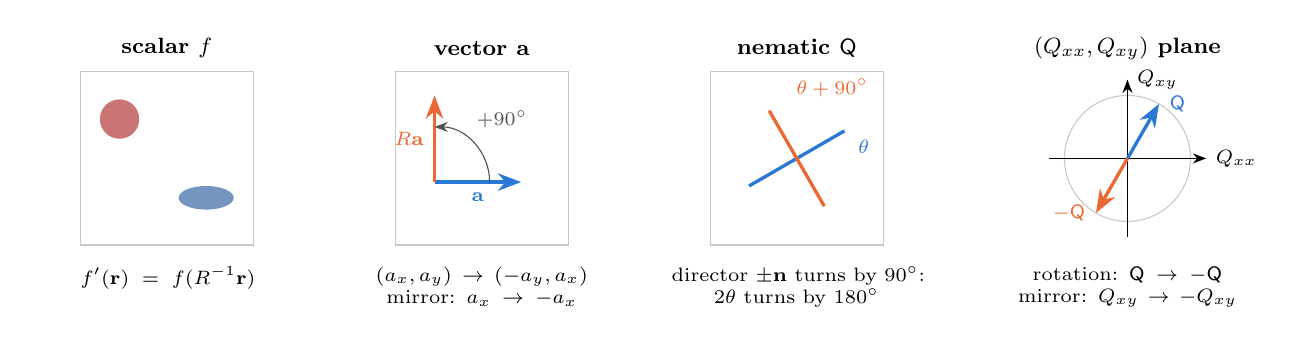
\begin{tikzpicture}[fig]
\tikzset{fcap/.style={small, text width=3.3cm, anchor=north}}
% scalar
\begin{scope}
  \node[lab] at (1.1,2.5) {scalar $f$};
  \draw[cGrid] (0,0) rectangle (2.2,2.2);
  \fill[cPos!70] (0.5,1.6) circle (0.25);  \fill[cNeg!60] (1.6,0.6) ellipse (0.35 and 0.15);
  \node[fcap] at (1.1,-0.15) {$f'(\mathbf r)=f(R^{-1}\mathbf r)$};
\end{scope}
% vector
\begin{scope}[shift={(4.0,0)}]
  \node[lab] at (1.1,2.5) {vector $\mathbf a$};
  \draw[cGrid] (0,0) rectangle (2.2,2.2);
  \draw[->, very thick, cP0] (0.5,0.8) -- (1.6,0.8) node[midway, below, small] {$\mathbf a$};
  \draw[->, very thick, cP1] (0.5,0.8) -- (0.5,1.9) node[midway, left, small] {$R\mathbf a$};
  \draw[->, cInk2] (1.2,0.8) arc (0:90:0.7) node[pos=0.6, above right, small] {$+90^\circ$};
  \node[fcap] at (1.1,-0.15) {$(a_x,a_y)\to(-a_y,a_x)$\\ mirror: $a_x\to-a_x$};
\end{scope}
% nematic
\begin{scope}[shift={(8.0,0)}]
  \node[lab] at (1.1,2.5) {nematic $\mathsf Q$};
  \draw[cGrid] (0,0) rectangle (2.2,2.2);
  \draw[very thick, cP0] ({1.1-0.7*cos(30)},{1.1-0.7*sin(30)}) -- ({1.1+0.7*cos(30)},{1.1+0.7*sin(30)});
  \draw[very thick, cP1] ({1.1-0.7*cos(120)},{1.1-0.7*sin(120)}) -- ({1.1+0.7*cos(120)},{1.1+0.7*sin(120)});
  \node[small, cP0] at (1.95,1.25) {$\theta$}; \node[small, cP1] at (1.55,2.0) {$\theta+90^\circ$};
  \node[fcap] at (1.1,-0.15) {director $\pm\mathbf n$ turns by $90^\circ$:\\ $2\theta$ turns by $180^\circ$};
\end{scope}
% the 2-theta plane
\begin{scope}[shift={(13.3,1.1)}]
  \node[lab] at (0,1.4) {$(Q_{xx},Q_{xy})$ plane};
  \draw[cGrid] (0,0) circle (0.8);
  \draw[->] (-1,0) -- (1.0,0) node[right, small] {$Q_{xx}$};
  \draw[->] (0,-1) -- (0,1.0) node[right, small] {$Q_{xy}$};
  \draw[->, very thick, cP0] (0,0) -- ({0.8*cos(60)},{0.8*sin(60)}) node[right, small] {$\mathsf Q$};
  \draw[->, very thick, cP1] (0,0) -- ({0.8*cos(240)},{0.8*sin(240)}) node[left, small] {$-\mathsf Q$};
  \node[fcap] at (0,-1.25) {rotation: $\mathsf Q\to-\mathsf Q$\\ mirror: $Q_{xy}\to-Q_{xy}$};
\end{scope}
\end{tikzpicture}

\caption{A rotation $R$ by $+90^\circ$ moves the grid and turns vectors and directors with
it. A director at angle $\theta$ is stored as $(Q_{xx},Q_{xy}) = \tfrac S2(\cos2\theta,\sin2\theta)$,
so turning it by $90^\circ$ turns $2\theta$ by $180^\circ$: $\mathsf Q\to-\mathsf Q$.}\label{fig:symmetry}
\end{figure}

\begin{tech}
The periodic square box has the symmetry group $D_4$ (four rotations by multiples of
$90^\circ$, each with or without a mirror), times the periodic translations (Fig.~\ref{fig:symmetry});
a non-periodic frame keeps only $D_4$ (Sec.~\ref{sec:frames}). Under the
rotation $R$ ($x$ towards $y$) and the mirror $M: x\to-x$ a field transforms as
\begin{align*}
\text{scalar: } & f'(\mathbf r)=f(R^{-1}\mathbf r), \\
\text{vector: } & \mathbf a'(\mathbf r)=R\,\mathbf a(R^{-1}\mathbf r),\quad (a_x,a_y)\to(-a_y,a_x);
  \qquad M:\ a_x\to-a_x, \\
\text{nematic: } & \mathsf Q'(\mathbf r)=R\,\mathsf Q(R^{-1}\mathbf r)R^{\mathsf T},\quad
  (Q_{xx},Q_{xy})\to(-Q_{xx},-Q_{xy}); \qquad M:\ Q_{xy}\to-Q_{xy}.
\end{align*}
The nematic rule follows from $\mathsf Q = S(\mathbf n\mathbf n-\tfrac12\mathbb I)$: a rotation by
$90^\circ$ adds $90^\circ$ to the angle of $\mathbf n$, hence $180^\circ$ to $2\theta$.

\emph{Physics parallel.} These are the transformation laws of tensors of rank 0, 1 and 2
under the point group of the lattice; a description built only from invariants of the group
(spectra on shells of $|\mathbf k|$, moments of $|\mathbf a|$, \ldots) is automatically
invariant, as a free energy built from scalar invariants of the order parameter is.
\end{tech}

\begin{codebox}
\textbf{Files.} \srcref{src/phasewall/fields.py}, \srcref{src/phasewall/io.py};
tests \srcref{tests/test_fields.py}, \srcref{tests/test_io.py}.

\code{Field(name, keys, kind, relative)}; \code{rotate90}, \code{mirror_x}, \code{transform},
\code{random_transform}. \code{load_ensemble} reads the TOML file; \code{read_snapshot}
reads HDF5 (and JLD2) files with h5py and transposes arrays written by Julia (column-major),
so that arrays are always indexed $[x, y]$ or $[x, y, \text{component}]$.

\textbf{Tests.} The vector rule is checked against an independent fact: the gradient of a
rotated scalar equals the rotated gradient. The nematic rule is checked by building
$\mathsf Q$ from a director field turned as a vector. Four turns and two mirrors give the
identity, and $M R M = R^{-1}$. Files written in the Julia layout read back unchanged.
\end{codebox}

%======================================================================
\section{Describing a snapshot}\label{sec:describe}
%======================================================================

\begin{figure}[H]
\centering
% Three blocks of descriptors: structure factor on shells, domains above a level, dynamics.
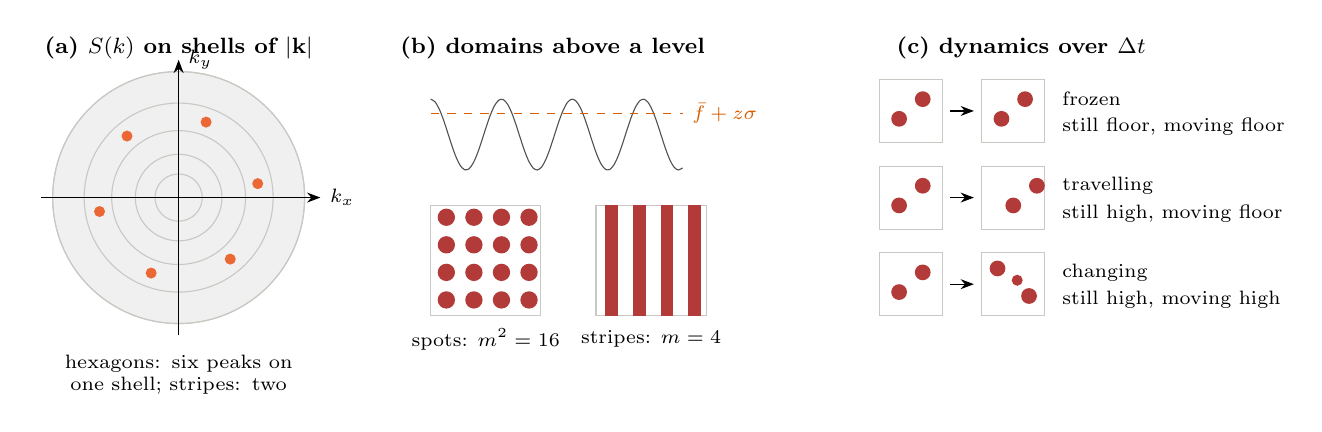
\begin{tikzpicture}[fig]
% (a) shells in k space
\begin{scope}
  \node[lab] at (0,1.9) {(a) $S(k)$ on shells of $|\mathbf k|$};
  \foreach \r/\c in {0.3/black!6, 0.55/black!10, 0.85/black!6, 1.2/black!10, 1.6/black!6}
    \draw[cGrid, fill=\c] (0,0) circle (\r);
  \foreach \r in {1.6, 1.2, 0.85, 0.55, 0.3} \draw[cGrid] (0,0) circle (\r);
  \foreach \t in {0,60,...,300} \fill[cP1] ({\t+10}:1.02) circle (0.07);
  \draw[->] (-1.75,0) -- (1.8,0) node[right, small] {$k_x$};
  \draw[->] (0,-1.75) -- (0,1.75) node[right, small] {$k_y$};
  \node[small, text width=3.6cm] at (0,-2.25) {hexagons: six peaks on one shell; stripes: two};
\end{scope}
% (b) domains above a level
\begin{scope}[shift={(3.2,-1.5)}]
  \node[lab] at (1.55,3.4) {(b) domains above a level};
  \draw[cGrid] (0,0) rectangle (1.4,1.4);
  \foreach \x in {0.2,0.55,0.9,1.25} \foreach \y in {0.2,0.55,0.9,1.25} \fill[cPos] (\x,\y) circle (0.11);
  \node[small] at (0.7,-0.3) {spots: $m^2=16$};
  \draw[cGrid] (2.1,0) rectangle (3.5,1.4);
  \foreach \x in {2.22,2.57,2.92,3.27} \fill[cPos] (\x,0) rectangle (\x+0.16,1.4);
  \node[small] at (2.8,-0.3) {stripes: $m=4$};
  \begin{scope}[shift={(0,1.75)}]
    \draw[domain=0:3.2, samples=60, smooth, cInk2] plot (\x, {0.55+0.45*cos(\x*400)});
    \draw[dashed, cAcc] (0,0.82) -- (3.2,0.82) node[right, small] {$\bar f+z\sigma$};
  \end{scope}
\end{scope}
% (c) dynamics
\begin{scope}[shift={(8.9,-1.5)}]
  \node[lab] at (1.8,3.4) {(c) dynamics over $\Delta t$};
  \foreach \row/\name/\sh/\st/\mv in {2.2/frozen/0/floor/floor, 1.1/travelling/0.15/high/floor, 0/changing/x/high/high} {
    \draw[cGrid] (0,\row) rectangle (0.8,\row+0.8);
    \fill[cPos] (0.25,\row+0.3) circle (0.1); \fill[cPos] (0.55,\row+0.55) circle (0.1);
    \draw[->] (0.9,\row+0.4) -- (1.2,\row+0.4);
    \draw[cGrid] (1.3,\row) rectangle (2.1,\row+0.8);
    \node[small, anchor=west] at (2.2,\row+0.55) {\name};
    \node[small, anchor=west] at (2.2,\row+0.2) {still \st, moving \mv};
  }
  \fill[cPos] (1.55,2.5) circle (0.1); \fill[cPos] (1.85,2.75) circle (0.1);
  \fill[cPos] (1.70,1.4) circle (0.1); \fill[cPos] (2.0,1.65) circle (0.1);
  \fill[cPos] (1.5,0.6) circle (0.1); \fill[cPos] (1.9,0.25) circle (0.1); \fill[cPos] (1.75,0.45) circle (0.07);
\end{scope}
\end{tikzpicture}

\caption{Three of the blocks. (a) The power spectrum is averaged over rings of $|\mathbf k|$,
so orientation does not matter. (b) Counting the domains above a level tells spots ($m^2$
domains) from stripes ($m$ domains, each closed through the periodic edge). (c) Two
correlations, at the same place and after the best shift, tell frozen, travelling and changing
patterns apart.}\label{fig:descriptors}
\end{figure}

\begin{tech}
Each field of each snapshot gives blocks of descriptors (Fig.~\ref{fig:descriptors}), none of which depends on the position or orientation of the pattern. For a field $a$ on an $N_x\times N_y$ periodic grid of spacing $\Delta x$ (components $a_c$;
$f=(\rho-\avg\rho)/\avg\rho$ for a ``relative'' scalar):

\textbf{amp:} $\log_{10}\sum_c \mathrm{var}(a_c)$, floored at $\log_{10}\epsilon_{\rm flat}^2=-12$.

\textbf{shape:} the structure factor
$S(k)=\frac{\Delta x^2}{N_xN_y}\avg{\textstyle\sum_c|\hat a_c(\mathbf k)|^2}_{|\mathbf k|\in\text{shell}}$,
divided by its sum. Shells start at half the lowest wavenumber $2\pi/L$, grow by a factor 1.2
but are never narrower than $2\pi/L$ (no empty shell), and end at $\pi/\Delta x$. Summing over
components makes $S$ invariant under a global rotation of vectors.

\textbf{mom:} mean (unless relative), standard deviation, skewness $\avg{z^3}$ and excess
kurtosis $\avg{z^4}-3$ of $v$, with $v=a$ (scalar), $|\mathbf a|$ (vector) or $2|\mathsf Q|=S$
(nematic). Skewness tells spots ($u>0$ peaks on a flat background) from stripes (symmetric).

\textbf{topo:} the number of connected domains (4-neighbour, periodic, per unit area) of
$\{v>\bar v+z\sigma\}$ and $\{v<\bar v+z\sigma\}$ for $z\in\{-1,0,1\}$.

\textbf{order} (vector, nematic): $|\avg{\mathbf a}|/\avg{|\mathbf a|}$, 1 for perfect alignment.

\textbf{flow} (vector): $\log_{10}\avg{(\nabla\!\cdot\!\mathbf a)^2}$,
$\log_{10}\avg{(\nabla\!\times\!\mathbf a)^2}$ and the curl share
$\avg{(\nabla\times\mathbf a)^2}/(\avg{(\nabla\cdot\mathbf a)^2}+\avg{(\nabla\times\mathbf a)^2})$
(spectral derivatives).

\textbf{dyn:} for a snapshot $y$ and the one $x$ taken $\Delta t$ earlier (fluctuations about
the mean), $C_{\rm still}=\sum xy/\sqrt{\sum x^2\sum y^2}$ and
$C_{\rm moving}=\max_{\mathbf T}\sum x(\mathbf r)\,y(\mathbf r+\mathbf T)/\sqrt{\sum x^2\sum y^2}$
(all periodic shifts $\mathbf T$, by FFT). Stored as $\log_{10}(1-C+10^{-3})$: the floor keeps
the round-off of a frozen pattern ($C=0.99999$) from looking like motion.

\emph{Physics parallel.} $S(k)$ is what a scattering experiment measures. The domain counts
are a discrete version of the Minkowski functionals (area, perimeter, Euler characteristic
of excursion sets) used for the topology of the cosmic microwave background and of
patterns in reaction-diffusion systems. Divergence and curl are the two halves of the
Helmholtz decomposition: splay against bend, asters against vortices. $C_{\rm still}$ and
$C_{\rm moving}$ are an intermediate scattering function at one lag, with and without
following the pattern (Lagrangian against Eulerian).
\end{tech}

\begin{figure}[H]
\centering
\includegraphics[width=0.62\textwidth]{data/sk_phases.pdf}
\caption{Shape of $S(k)$ at the central point of each phase of the demo. Stripes and hexagons
both peak at $k=1$, the wavenumber selected by the Swift-Hohenberg operator; hexagons are
narrower. The uniform state's residual noise also decays fastest away from $k=1$, so its
\emph{shape} is similar: it is the amplitude block that separates it (median $\log_{10}$
variance at the floor $-12$, against $-0.4$ for stripes and $-0.7$ for hexagons).}
\end{figure}

\begin{codebox}
\textbf{Files.} \srcref{src/phasewall/describe.py}; tests \srcref{tests/test_describe.py}.

Columns are named \code{field.block.name} (for example \code{u.shape.k07}).
\code{describe_ensemble(ens, workers)} returns one row per snapshot (the last \code{last}
snapshots of each run), plus the list of runs that could not be read. It uses
\code{concurrent.futures.ProcessPoolExecutor} for parallel reading; keep 2 or 3 workers
over a network share. Domains are labelled with \code{scipy.ndimage.label} and joined across
the periodic edges by a union-find.

\textbf{Tests} (known answers): $S(k)$ of $\cos(k_0x)$ has all its power in the shell of $k_0$;
two-valued fields give the exact skewness $2/\sqrt3$ and kurtosis $-2/3$; $\cos kx+\cos ky$
gives $m^2$ domains and $\cos kx$ gives $m$; a gradient has curl share 0 and its rotation by
$90^\circ$ curl share 1; a frozen pattern gives both correlations at the floor, a shifted one
only $C_{\rm moving}$; and every descriptor of random scalar, vector and nematic fields is
unchanged under all 8 elements of $D_4$ and periodic shifts.
\end{codebox}

\subsection{Frames: crops, coarsening and non-periodic boxes}\label{sec:frames}

\begin{figure}[H]
\centering
% (a) crop of side Lc in a non-periodic box, margin s; (b) the frame at t slid over the frame
% at t - dt extended by s; (c) Tukey window along one side.
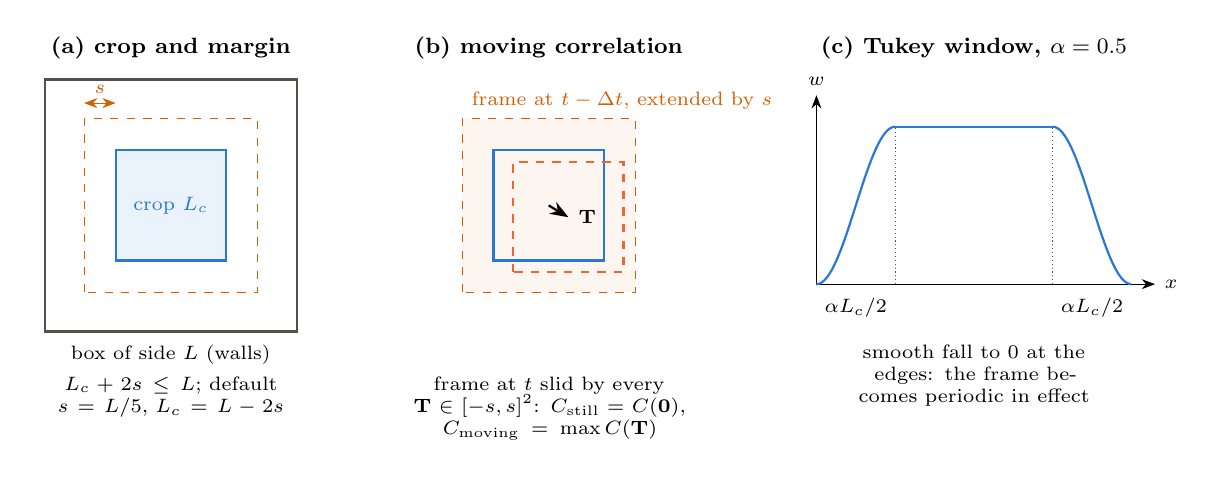
\begin{tikzpicture}[fig]
\begin{scope}
  \node[lab] at (1.6,3.6) {(a) crop and margin};
  \draw[thick, cInk2] (0,0) rectangle (3.2,3.2);
  \node[small, anchor=north] at (1.6,-0.05) {box of side $L$ (walls)};
  \draw[cAcc, dashed] (0.5,0.5) rectangle (2.7,2.7);
  \draw[thick, cP0, fill=cP0!10] (0.9,0.9) rectangle (2.3,2.3);
  \node[small, cP0] at (1.6,1.6) {crop $L_c$};
  \draw[<->, cAcc] (0.5,2.9) -- (0.9,2.9) node[midway, above, small] {$s$};
  \node[small, text width=3.4cm, anchor=north] at (1.6,-0.45) {$L_c+2s\le L$; default\\ $s=L/5$, $L_c=L-2s$};
\end{scope}
\begin{scope}[shift={(4.8,0)}]
  \node[lab] at (1.6,3.6) {(b) moving correlation};
  \draw[cAcc, dashed, fill=cAcc!6] (0.5,0.5) rectangle (2.7,2.7);
  \node[small, cAcc, anchor=south west] at (0.5,2.7) {frame at $t-\Delta t$, extended by $s$};
  \draw[thick, cP0] (0.9,0.9) rectangle (2.3,2.3);
  \draw[thick, cP1, dashed] (1.15,0.75) rectangle (2.55,2.15);
  \draw[->, thick] (1.6,1.6) -- (1.85,1.45) node[right, small] {$\mathbf T$};
  \node[small, text width=3.6cm, anchor=north] at (1.6,-0.45) {frame at $t$ slid by every
    $\mathbf T\in[-s,s]^2$: $C_{\rm still}=C(\mathbf 0)$, $C_{\rm moving}=\max C(\mathbf T)$};
\end{scope}
\begin{scope}[shift={(9.8,0.6)}]
  \node[lab] at (2.0,3.0) {(c) Tukey window, $\alpha=0.5$};
  \draw[->] (0,0) -- (4.3,0) node[right, small] {$x$};
  \draw[->] (0,0) -- (0,2.4) node[above, small] {$w$};
  \draw[thick, cP0, domain=0:1, samples=40, smooth] plot (\x, {1.0*(1-cos(180*\x))});
  \draw[thick, cP0] (1,2) -- (3,2);
  \draw[thick, cP0, domain=3:4, samples=40, smooth] plot (\x, {1.0*(1-cos(180*(4-\x)))});
  \draw[densely dotted, cInk2] (1,0) -- (1,2); \draw[densely dotted, cInk2] (3,0) -- (3,2);
  \node[small] at (0.5,-0.3) {$\alpha L_c/2$}; \node[small] at (3.5,-0.3) {$\alpha L_c/2$};
  \node[small, text width=3.6cm, anchor=north] at (2.0,-0.65) {smooth fall to 0 at the edges:
    the frame becomes periodic in effect};
\end{scope}
\end{tikzpicture}

\caption{(a) A crop of a non-periodic box keeps a margin $s$ (\code{max_shift}) from the walls.
(b) The moving correlation slides the frame at $t$ over the frame at $t-\Delta t$ extended by
$s$. (c) The window that makes a non-periodic frame periodic in effect for $S(k)$.}\label{fig:frames}
\end{figure}

\begin{tech}
\textbf{Why frames.} The shells of $S(k)$ start from the side of the frame, so frames of
different sizes give columns at different wavenumbers, and domain counts depend a little on
the grid spacing ($33$ against $31$ low-$|\mathbf p|$ domains when $\Delta x$ is halved, same
pattern). Every run is therefore described on a frame of the same physical side $L_c$
(\code{crop}) and the same spacing (\code{dx_target}, by block averaging over $f\times f$ points,
$f=$ \code{dx_target}$/\Delta x$ an integer). A whole periodic box is described as it is; a crop,
or any frame of a non-periodic box, is not periodic (Fig.~\ref{fig:frames}a). Runs whose
frames would give different shells are refused with an error. Only rotations and mirrors
remain symmetries of a non-periodic frame; the descriptors are tested for invariance under
those eight.

\textbf{$S(k)$ of a non-periodic frame.} The FFT treats the frame as periodic, so the jump
between opposite edges leaks power $\propto k^{-2}$ to all wavenumbers; a mirror extension
removes the jump but keeps a kink in the slope and leaks almost as much. \pw{} multiplies the
fluctuations by a separable Tukey window $w(x)w(y)$ (Fig.~\ref{fig:frames}c),
\[
w(x)=\begin{cases}\tfrac12\big[1-\cos(2\pi x/\alpha L_c)\big], & x<\alpha L_c/2,\\
1, & \alpha L_c/2\le x\le L_c(1-\alpha/2),\\ \text{symmetric}, & \text{otherwise},\end{cases}
\qquad \alpha=0.5,
\]
divides the power by $\avg{w^2}$, and keeps only the shells with $k\ge 2\pi m/L_c$
(\code{min_wavelengths} $m=3$): a frame cannot measure wavelengths comparable to its side.
Crops of 48 points cut from 24 periodic random fields with a known broadband spectrum give
(ratio crop / exact, mean of 480 crops):
\begin{center}\small
\begin{tabular}{@{}lcccccccc@{}}
\toprule
wavelength & $L_c$ & $L_c/2$ & $L_c/3$ & $L_c/5$ & $L_c/8$ & $L_c/11$ & $L_c/12$ & $L_c/13$ \\
\midrule
ratio & 1.33 & 1.15 & 1.01 & 0.98 & 0.97 & 1.02 & 1.06 & 1.12 \\
\bottomrule
\end{tabular}
\end{center}
Beyond $L_c/11$, where the spectrum has fallen below a tenth of its peak, the remaining edge
leakage grows. On crops of Swift-Hohenberg patterns the share of power outside the peak is
5\% without window (or with a mirror extension) and 1.2\% with the window.

\textbf{Derivatives.} $\partial_xa\simeq[a(x+\Delta x)-a(x-\Delta x)]/2\Delta x$ on the interior
points (second order).

\textbf{Moving correlation.} With $y$ the frame at $t$ ($n$ points, mean removed) and $x$ the
frame at $t-\Delta t$ extended by $s$ points on every side (Fig.~\ref{fig:frames}b),
\[
C(\mathbf T)=\frac{\sum_{\mathbf r}y(\mathbf r)\,x(\mathbf r+\mathbf T)}
{\sqrt{\sum_{\mathbf r}y^2\;\Big[\sum_{\mathbf r}x(\mathbf r+\mathbf T)^2-\tfrac1n\big(\sum_{\mathbf r}x(\mathbf r+\mathbf T)\big)^2\Big]}},
\qquad \mathbf T\in[-s,s]^2,
\]
the Pearson correlation of the frame with the window under it. The three sums over windows
are computed for all shifts at once by FFT convolutions (fast normalised cross-correlation,
Lewis 1995), so the cost hardly depends on $s$. $C_{\rm still}=C(\mathbf 0)$,
$C_{\rm moving}=\max_{\mathbf T}C(\mathbf T)$. A pattern that moves by more than $s$ during
$\Delta t$ is seen as changing. In a periodic box the margin wraps around; in a non-periodic
one the crop stays $s$ away from the walls (by default $s=L/5$ and $L_c=L-2s$).

\emph{Physics parallel.} The window is the apodisation of spectroscopy and of finite-time
Fourier analysis: a sharp truncation (a box window) gives the $\mathrm{sinc}^2$ side lobes of
single-slit diffraction; a smooth aperture suppresses them at the price of a slightly wider
central peak. The moving correlation is particle image velocimetry: the displacement of a
pattern is the shift that maximises the correlation of two interrogation windows.
\end{tech}

\begin{codebox}
\textbf{Files.} \srcref{src/phasewall/frames.py} (\code{frame_for}, \code{coarsen}, \code{cut},
\code{prepare}), \srcref{src/phasewall/describe.py} (\code{window}, \code{structure_factor},
\code{div_curl}, \code{correlations} with \code{scipy.signal.fftconvolve}, \code{run_frame});
tests \srcref{tests/test_frames.py}. Keys of \code{[ensemble]}: \code{periodic}, \code{crop},
\code{dx_target}, \code{max_shift}, \code{min_wavelengths}; per-run grid spacing as a column
\code{dx} of the table of runs. Unknown keys are errors.

\textbf{Tests.} Crop sizes, margins and errors; block averaging of constant blocks; $S(k)$ of
crops within 6\% of the exact one from $L_c/3$ to $L_c/11$ (the table above); finite against
spectral derivatives; a frame moved by $(3,-2)$ points gives $C_{\rm moving}$ at the floor and a
move of 9 points with $s=5$ does not; invariance under the eight rotations and mirrors; the
same descriptors (except domain counts) at $\Delta x$ and at $\Delta x/2$ coarsened to $\Delta x$;
mixed grids refused without a common frame and accepted with one.
\end{codebox}

\subsection{A learned description: a convolutional encoder}\label{sec:learned}

\begin{figure}[H]
\centering
% The learned description: two views of a run -> f -> h -> g -> z; InfoNCE on the sphere.
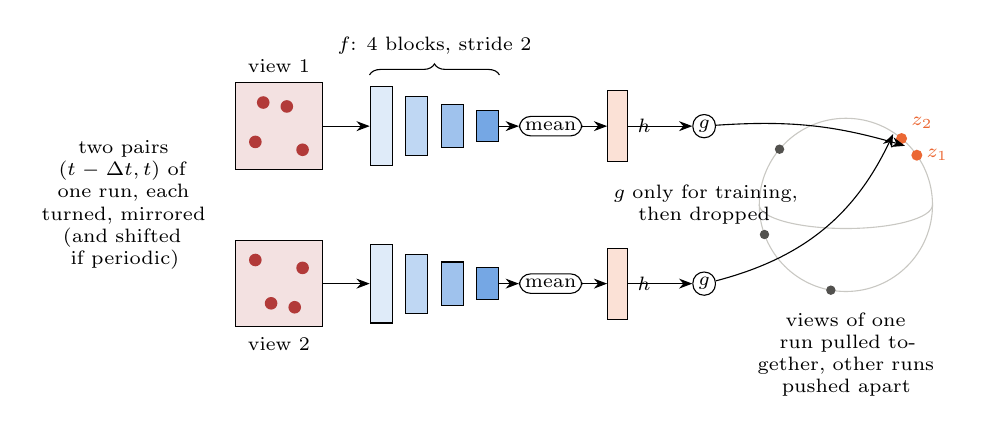
\begin{tikzpicture}[fig, node distance=0.35cm]
\tikzset{map/.style={draw, fill=#1, minimum height=1.1cm, minimum width=0.28cm, inner sep=0pt},
         op/.style={draw, rounded corners, font=\scriptsize, align=center, inner sep=2pt}}
% view 1
\node[draw, fill=cPos!15, minimum size=1.1cm, label={[small]above:view 1}] (v1) at (0,1.0) {};
\foreach \x/\y in {-0.3/-0.2, 0.1/0.25, 0.3/-0.3, -0.2/0.3} \fill[cPos] ($(v1)+(\x,\y)$) circle (0.08);
\node[draw, fill=cPos!15, minimum size=1.1cm, label={[small]below:view 2}] (v2) at (0,-1.0) {};
\foreach \x/\y in {0.3/0.2, -0.1/-0.25, -0.3/0.3, 0.2/-0.3} \fill[cPos] ($(v2)+(\x,\y)$) circle (0.08);
\node[small, text width=2.2cm, anchor=east] at (-0.75,0) {two pairs $(t-\Delta t,t)$ of one run, each turned, mirrored (and shifted if periodic)};
% encoder f
\foreach \v/\yy in {v1/1.0, v2/-1.0} {
  \node[map=cP0!15, minimum height=1.0cm] (a\v) at (1.3,\yy) {};
  \node[map=cP0!30, minimum height=0.75cm] (b\v) at (1.75,\yy) {};
  \node[map=cP0!45, minimum height=0.55cm] (c\v) at (2.2,\yy) {};
  \node[map=cP0!65, minimum height=0.4cm] (d\v) at (2.65,\yy) {};
  \draw[->] (\v) -- (a\v);
  \node[op] (m\v) at (3.45,\yy) {mean};
  \draw[->] (d\v) -- (m\v);
  \node[draw, fill=cP1!20, minimum width=0.25cm, minimum height=0.9cm, label={[small]right:$h$}] (h\v) at (4.3,\yy) {};
  \draw[->] (m\v) -- (h\v);
  \node[op] (g\v) at (5.4,\yy) {$g$};
  \draw[->] (h\v) -- (g\v);
}
\draw[decorate, decoration={brace, amplitude=4pt}] (1.15,1.65) -- (2.8,1.65) node[midway, above=4pt, small] {$f$: 4 blocks, stride 2};
% sphere
\begin{scope}[shift={(7.2,0)}]
  \draw[cGrid] (0,0) circle (1.1);
  \draw[cGrid] (-1.1,0) arc (180:360:1.1 and 0.3);
  \fill[cP1] (35:1.1) circle (0.07) node[right, small] {$z_1$};
  \fill[cP1] (50:1.1) circle (0.07) node[above right, small] {$z_2$};
  \fill[cInk2] (200:1.1) circle (0.06); \fill[cInk2] (260:1.1) circle (0.06); \fill[cInk2] (140:1.1) circle (0.06);
  \node[small, text width=2.6cm, anchor=north] at (0,-1.25) {views of one run pulled together, other runs pushed apart};
\end{scope}
\draw[->] (gv1) to[bend left=10] (7.95,0.75);
\draw[->] (gv2) to[bend right=25] (7.8,0.9);
\node[small, text width=2.3cm, align=center] at (5.4,0) {$g$ only for training, then dropped};
\end{tikzpicture}

\caption{The learned description. Two views of one run go through the same encoder $f$
(four convolution blocks that halve the grid, then the mean over the frame) and give $h$;
the head $g$ maps $h$ to a point $z$ on the unit sphere, where the loss pulls the two views of
a run together and pushes other runs away. After training only $f$ is kept: $h$ replaces the
hand-made $\mathbf x$ in the walls method, which is unchanged.}\label{fig:cnn}
\end{figure}

\begin{tech}
\textbf{Two describers, one method.} The walls method needs one vector per snapshot. The
hand-made $f$ (Sec.~\ref{sec:describe}) computes it with fixed formulas and has nothing to
learn. The learned $f$ (Fig.~\ref{fig:cnn}) is a convolutional network trained on the
ensemble itself, without labels. Its output $h$ (256 numbers) is written as a table of the
same format (columns \code{cnn.h.d000} \ldots), so steps 3 to 5 run on it unchanged.

\textbf{Input.} A sample is a pair of frames of one run, at $t-\Delta t$ and $t$ (the frames of
Sec.~\ref{sec:frames}: same crop and coarsening as the hand-made description). Each field
gives one channel (scalar) or two (vector, nematic); each field is divided by one number, its
r.m.s.\ value over the ensemble, shared by its components so that rotations act on them as on
the field.

\textbf{Encoder.} Four blocks, each a $3\times3$ convolution with stride 2 then a $3\times3$
convolution, each followed by batch normalisation and $\mathrm{ReLU}(u)=\max(u,0)$; channels
$32,64,128,256$. The receptive field (points of the input that one output value sees) grows as
$7,19,43,91$ points over the four blocks, larger than the $64$-point demo box. Then
$h_c=\frac{1}{|\Omega|}\sum_{\mathbf r\in\Omega}F_c(\mathbf r)$, the mean of each final map
$F_c$ over the frame $\Omega$. Padding is circular for a periodic frame, so a shift of the input by a
multiple of $2^4=16$ points leaves $h$ exactly unchanged (tested); zero padding otherwise.
Invariance under rotations and mirrors is not built in: it is learned from the augmentations.

\textbf{Training (SimCLR).} A batch holds two views of each of $N$ runs: two different pairs of
the run, each turned by a random element of $D_4$ with the rules of Sec.~\ref{sec:fields}
(and shifted at random in a periodic frame). With $z=g(h)/|g(h)|$, $g$ a two-layer perceptron,
the InfoNCE loss is
\[
\mathcal L=-\frac{1}{2N}\sum_{i=1}^{2N}\log\frac{e^{z_i\cdot z_{i^+}/T}}{\sum_{k\ne i}e^{z_i\cdot z_k/T}},\qquad T=0.2,
\]
with $i^+$ the other view of the same run: each view must recognise its partner among the
$2N-1$ others. If all $z$ are equal (collapse), $\mathcal L=\ln(2N-1)=5.54$ for $N=128$.
AdamW, learning rate $10^{-3}$ with a linear warm-up over 3 epochs then a cosine decay, 40
epochs, every run drawn 4 times per epoch. Checks logged each epoch: alignment (mean
$z_i\cdot z_{i^+}$), uniformity ($\log\avg{e^{-2|z_i-z_k|^2}}$ over different runs) and the
effective rank of $h$ ($e^{S}$ with $S$ the entropy of the normalised singular values).

\emph{Physics parallel.} The fraction in $\mathcal L$ is a Boltzmann probability at
temperature $T$ with energy $-z_i\cdot z_k$: the loss is the free energy cost of finding the
partner. Minimising it balances an attraction between partners (alignment) and a repulsion
between all points on the sphere (uniformity), as charges spread on a sphere in the Thomson
problem; collapse is the state without repulsion. The stride-2 blocks coarse-grain the field
step by step, as in a real-space renormalisation group, but with learned kernels.
\end{tech}

\begin{codebox}
\textbf{Files.} \srcref{src/phasewall/nn/data.py} (\code{load_frames}, \code{augment},
\code{PairViews}), \srcref{src/phasewall/nn/model.py} (\code{Encoder}, \code{ProjectionHead}),
\srcref{src/phasewall/nn/loss.py} (\code{info_nce}, \code{alignment}, \code{uniformity},
\code{effective_rank}), \srcref{src/phasewall/nn/train.py} (\code{Settings}, \code{train},
\code{embed}, \code{h_table}, \code{save}, \code{load}); tests \srcref{tests/test_nn.py}; extra
\code{[nn]} (PyTorch; Apple GPU, CUDA or CPU).
Commands: \code{phasewall learn ensemble.toml} trains and writes \code{encoder/descriptors_cnn.csv};
\code{phasewall describe ensemble.toml --encoder encoder} describes another ensemble with it;
\code{phasewall walls} then reads either table.

\textbf{Tests.} Augmentations equal \code{fields.transform}; $h$ unchanged by circular shifts
of 16 points and changed by 5; the loss is $\ln(2N-1)$ at collapse and $\approx0$ for perfect
pairs; a 6-epoch training separates stripes from spots ($h$ farther between kinds than within);
saving and loading give the same $h$; the two commands give the same table.
\end{codebox}

%======================================================================
\section{Comparing parameter points}\label{sec:compare}
%======================================================================

\subsection{Features}

\begin{tech}
$x_{ij}\to(x_{ij}-\bar x_j)/\sigma_j$; constant columns are dropped, missing values (dynamics
of a snapshot without partner) set to the column median. A block $b$ of $n_b$ columns is
divided by $\sqrt{n_b}$, so its expected contribution to a squared Euclidean distance is the
same for every block.
\end{tech}

\subsection{Energy distance between two samples}

\begin{figure}[H]
\centering
% Energy distance between two samples, and its electrostatic picture.
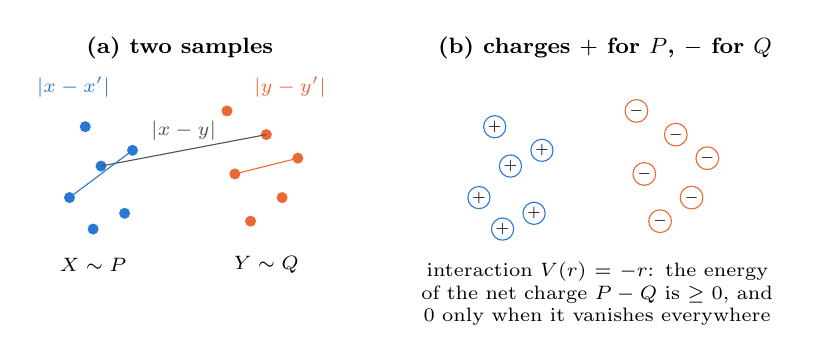
\begin{tikzpicture}[fig]
\begin{scope}
  \node[lab] at (1.6,2.4) {(a) two samples};
  \foreach \x/\y in {0.2/0.5, 0.6/0.9, 0.4/1.4, 0.9/0.3, 1.0/1.1, 0.5/0.1} \fill[cP0] (\x,\y) circle (0.07);
  \foreach \x/\y in {2.3/0.8, 2.7/1.3, 2.9/0.5, 2.5/0.2, 3.1/1.0, 2.2/1.6} \fill[cP1] (\x,\y) circle (0.07);
  \draw[cInk2] (0.6,0.9) -- (2.7,1.3) node[pos=0.5, above, small] {$|x-y|$};
  \draw[cP0] (0.2,0.5) -- (1.0,1.1); \node[small, cP0] at (0.25,1.9) {$|x-x'|$};
  \draw[cP1] (2.3,0.8) -- (3.1,1.0); \node[small, cP1] at (3.0,1.9) {$|y-y'|$};
  \node[small] at (0.5,-0.35) {$X\sim P$}; \node[small] at (2.7,-0.35) {$Y\sim Q$};
\end{scope}
\begin{scope}[shift={(5.2,0)}]
  \node[lab] at (1.8,2.4) {(b) charges $+$ for $P$, $-$ for $Q$};
  \foreach \x/\y in {0.2/0.5, 0.6/0.9, 0.4/1.4, 0.9/0.3, 1.0/1.1, 0.5/0.1}
    \node[circle, draw=cP0, inner sep=0.5pt, font=\tiny] at (\x,\y) {$+$};
  \foreach \x/\y in {2.3/0.8, 2.7/1.3, 2.9/0.5, 2.5/0.2, 3.1/1.0, 2.2/1.6}
    \node[circle, draw=cP1, inner sep=0.5pt, font=\tiny] at (\x,\y) {$-$};
  \node[small, text width=4.6cm, anchor=north] at (1.7,-0.2) {interaction $V(r)=-r$: the energy of the net charge
    $P-Q$ is $\ge 0$, and $0$ only when it vanishes everywhere};
\end{scope}
\end{tikzpicture}

\caption{(a) The energy distance compares distances across the two samples with distances
inside each. (b) It is the energy of charges $+$ (sample $P$) and $-$ (sample $Q$) that
interact through $V(r)=-r$.}\label{fig:energy}
\end{figure}

\begin{tech}
The runs of a point form a sample in descriptor space; neighbouring points are compared through their whole distributions, not only their means (a bistable point and a pure one may have the same mean). For samples $X\sim P$ and $Y\sim Q$ in $\mathbb R^d$ (Sz\'ekely and Rizzo; Fig.~\ref{fig:energy}a),
\[
D^2(P,Q)=2\,\mathbb E|X-Y|-\mathbb E|X-X'|-\mathbb E|Y-Y'|
=\frac{1}{c_d}\int_{\mathbb R^d}\frac{|\varphi_P(\mathbf t)-\varphi_Q(\mathbf t)|^2}{|\mathbf t|^{d+1}}\,d\mathbf t\;\ge0,
\]
with $\varphi$ the characteristic functions: $D=0$ if and only if $P=Q$. \pw{} estimates
$D^2$ with the unbiased U-statistic (the within-sample averages leave out $i=j$), which
comes out negative about half of the time when $P=Q$; \code{energy_statistic} returns it as
it is, and \code{energy_distance} returns $\sqrt{\max(D^2,0)}$.

\emph{Physics parallel} (Fig.~\ref{fig:energy}b). Put a charge $+1/n$ on every point of $X$ and $-1/m$ on every point
of $Y$, interacting through $V(r)=-r$. Then $D^2=-\iint|\mathbf x-\mathbf y|\,d\mu(\mathbf x)\,d\mu(\mathbf y)$
with $\mu=P-Q$ is the interaction energy of a \emph{neutral} charge distribution. As the
Coulomb energy of a neutral distribution is positive and vanishes only when the charge
density is zero everywhere, $D^2\ge0$ with equality only for $P=Q$: the kernel $-r$ is
conditionally positive definite, as $1/r$ is positive definite.
\end{tech}

\subsection{Halves, spread and jumps}

\begin{figure}[H]
\centering
% Halves of two neighbouring points: spread, jump, and the two independent jumps J1 and J2.
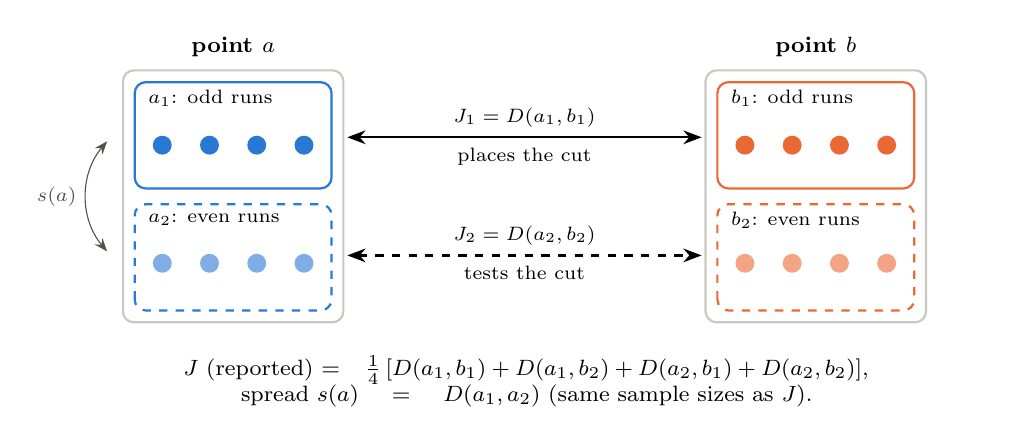
\begin{tikzpicture}[fig]
\foreach \name/\x/\c in {a/0/cP0, b/7.4/cP1} {
  \draw[rounded corners, cGrid, thick] (\x-1.4,-1.6) rectangle (\x+1.4,1.6);
  \node[lab] at (\x,1.9) {point $\name$};
  \draw[rounded corners, \c, thick] (\x-1.25,0.1) rectangle (\x+1.25,1.45);
  \draw[rounded corners, \c, thick, dashed] (\x-1.25,-1.45) rectangle (\x+1.25,-0.1);
  \node[small, anchor=west] at (\x-1.2,1.25) {$\name_1$: odd runs};
  \node[small, anchor=west] at (\x-1.2,-0.3) {$\name_2$: even runs};
  \foreach \i in {0,...,3} {
    \fill[\c] (\x-0.9+0.6*\i,0.65) circle (0.12);
    \fill[\c!60] (\x-0.9+0.6*\i,-0.85) circle (0.12);
  }
}
\draw[<->, thick] (1.45,0.75) -- node[above, small] {$J_1=D(a_1,b_1)$} node[below, small] {places the cut} (5.95,0.75);
\draw[<->, thick, dashed] (1.45,-0.75) -- node[above, small] {$J_2=D(a_2,b_2)$} node[below, small] {tests the cut} (5.95,-0.75);
\draw[<->, cInk2] (-1.6,0.7) to[bend right=40] node[left, small] {$s(a)$} (-1.6,-0.7);
\node[note, text width=12cm] at (3.7,-2.35) {$J$ (reported) $=\frac14\left[D(a_1,b_1)+D(a_1,b_2)+D(a_2,b_1)+D(a_2,b_2)\right]$,
  \quad spread $s(a)=D(a_1,a_2)$ (same sample sizes as $J$).};
\end{tikzpicture}

\caption{Spread, jump and the two independent jumps of a link. In the demo each half holds 4
of the 8 runs of a point.}\label{fig:halves}
\end{figure}

\begin{tech}
Each point is split into two halves (Fig.~\ref{fig:halves}): alternate runs, or earlier and
later snapshots when it has a single run. The spread $s(a)=D(a_1,a_2)$ measures noise; the
jump $J$ averages the four distances between halves of two neighbours, so jump and spread
compare samples of the same size. $J_1$ and $J_2$ use different runs; their roles are
given in Sec.~\ref{sec:test}.

Graph: nodes are the distinct parameter points (rounded to 9 decimals); two nodes are linked
when all parameters but one are equal and they are consecutive along that one, among all
nodes of the scan. A refined line therefore links to the coarse points around it.

Jumps below the \emph{floor} (10\% quantile of the positive spreads) are set to the floor: in
$\log J$, differences between two values that are both at noise level are meaningless.
At most 200 snapshots per point are used (drawn at random).
\end{tech}

\begin{codebox}
\textbf{Files.} \srcref{src/phasewall/walls.py} (\code{feature_matrix},
\code{energy_statistic}, \code{energy_distance}, \code{halves}, \code{jump},
\code{half_jumps}), \srcref{src/phasewall/graph.py} (\code{parameter_nodes},
\code{grid_edges}); tests \srcref{tests/test_walls.py}, \srcref{tests/test_graph.py}.
Distances with \code{scipy.spatial.distance.cdist}.

\textbf{Tests.} Energy distance near 0 for two samples of one Gaussian, near
$\sqrt{2s-2\cdot1.6}$ for a shift $s=3$ and growing with $s$; halves by run or by time;
block weighting gives each block of 4 columns a standard deviation $1/2$; the links of a full
$3\times2$ grid and of a refined line are listed exactly.
\end{codebox}

%======================================================================
\section{Cuts: where a random walk is slowed down}\label{sec:cuts}
%======================================================================

\begin{figure}[H]
\centering
% (a) the scan graph with weights; (b) physics parallel: double well, ground state and slowest mode.
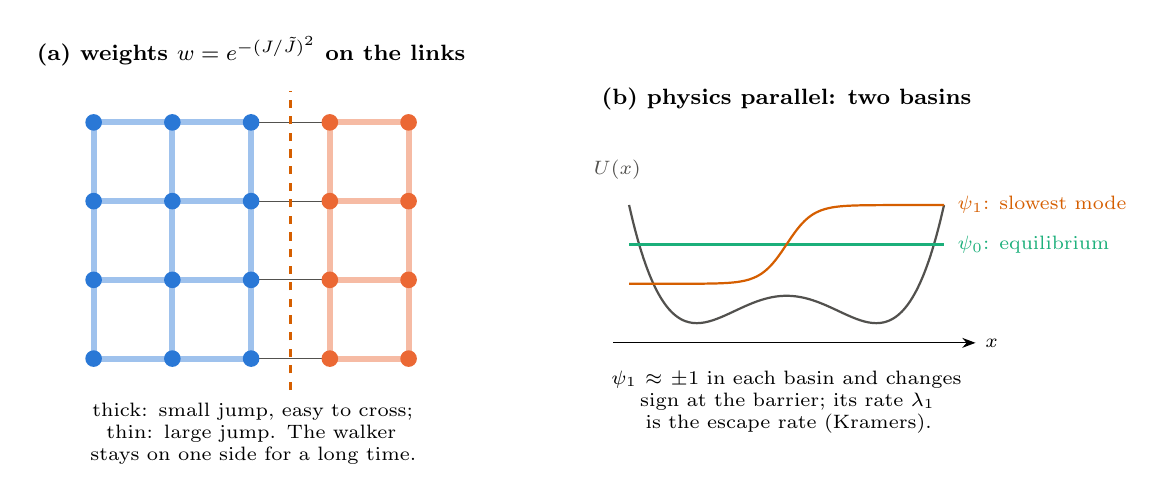
\begin{tikzpicture}[fig]
\begin{scope}
  \node[lab] at (2.0,3.9) {(a) weights $w=e^{-(J/\tilde J)^2}$ on the links};
  % links: thick inside each side, thin across the wall between columns 2 and 3
  \foreach \j in {0,...,3} {
    \foreach \i in {0,1} \draw[line width=2.2pt, cP0!45] (\i,\j) -- (\i+1,\j);
    \foreach \i in {3} \draw[line width=2.2pt, cP1!45] (\i,\j) -- (\i+1,\j);
    \draw[line width=0.3pt, cInk2] (2,\j) -- (3,\j);
  }
  \foreach \i in {0,1,2} \foreach \j in {0,1,2} \draw[line width=2.2pt, cP0!45] (\i,\j) -- (\i,\j+1);
  \foreach \i in {3,4} \foreach \j in {0,1,2} \draw[line width=2.2pt, cP1!45] (\i,\j) -- (\i,\j+1);
  \foreach \i in {0,1,2} \foreach \j in {0,...,3} \node[dot=cP0, minimum size=6pt] at (\i,\j) {};
  \foreach \i in {3,4} \foreach \j in {0,...,3} \node[dot=cP1, minimum size=6pt] at (\i,\j) {};
  \draw[wall, dashed] (2.5,-0.4) -- (2.5,3.4);
  \node[small, text width=4.6cm] at (2,-0.95) {thick: small jump, easy to cross;
    thin: large jump. The walker stays on one side for a long time.};
\end{scope}
\begin{scope}[shift={(6.6,0.2)}]
  \node[lab] at (2.2,3.1) {(b) physics parallel: two basins};
  \draw[->] (0,0) -- (4.6,0) node[right, small] {$x$};
  \draw[thick, cInk2, domain=0.2:4.2, samples=80, smooth] plot (\x, {0.35*((\x-2.2)^2-1.3)^2/1.7+0.25});
  \node[small, cInk2] at (0.05,2.2) {$U(x)$};
  \draw[cP2, thick, domain=0.2:4.2, samples=60, smooth] plot (\x, {1.25+0.0*\x});
  \node[small, cP2, anchor=west] at (4.25,1.25) {$\psi_0$: equilibrium};
  \draw[cAcc, thick, domain=0.2:4.2, samples=80, smooth] plot (\x, {1.25+0.5*tanh(3*(\x-2.2))});
  \node[small, cAcc, anchor=west] at (4.25,1.75) {$\psi_1$: slowest mode};
  \node[small, text width=4.8cm] at (2.2,-0.75) {$\psi_1\approx\pm1$ in each basin and changes sign at the barrier;
    its rate $\lambda_1$ is the escape rate (Kramers).};
\end{scope}
\end{tikzpicture}

\caption{(a) Links weighted by their jumps: across a wall the weights are small. (b) The same
mathematics as diffusion in a double well: the slowest mode separates the two basins.}\label{fig:spectral}
\end{figure}

\begin{tech}
Each link (Fig.~\ref{fig:spectral}a) gets the weight $W_{ab}=\max\!\big(e^{-(J_1/\tilde J_1)^2},10^{-8}\big)$, with
$\tilde J_1$ the median of $J_1$ over all links (the lower bound keeps the graph connected
across very strong walls). With the degrees $d_a=\sum_bW_{ab}$, the random walk
$P=d^{-1}W$ and the normalised Laplacian $L=\mathbb I-d^{-1/2}Wd^{-1/2}$ have the same
spectrum up to $\lambda\to1-\lambda$: a mode of eigenvalue $\lambda$ of $L$ decays as
$(1-\lambda)^t$. $\lambda_0=0$ is the stationary state ($\propto d$); the second eigenvalue
$\lambda_1$ (the Fiedler value) is the slowest relaxation, and its eigenvector
$\mathbf v=d^{-1/2}\mathbf u_1$ orders the points across the strongest barrier.

The points are sorted by $\mathbf v$; for each prefix $S$ (with at least \code{MIN_PHASE}=3
points on each side) the normalised cut (Shi and Malik 2000)
\[
\mathrm{Ncut}(S)=\frac{\cut(S,\bar S)}{\vol(S)}+\frac{\cut(S,\bar S)}{\vol(\bar S)},\qquad
\cut(S,\bar S)=\sum_{a\in S,b\in\bar S}W_{ab},\quad \vol(S)=\sum_{a\in S}d_a
\]
is computed, and the smallest one is the proposed cut (both steps on the demo: Fig.~\ref{fig:fiedler}). The Cheeger inequality
$\lambda_1/2\le h\le\sqrt{2\lambda_1}$ ($h$ the best conductance) says that a small
$\lambda_1$ means a good cut exists.

\emph{Physics parallel} (Fig.~\ref{fig:spectral}b). For an overdamped particle in a potential $U$ with two basins, the
Fokker-Planck operator has $\lambda_0=0$ (Boltzmann distribution) and a small $\lambda_1$,
the Kramers escape rate $\propto e^{-\Delta U/k_BT}$; its eigenfunction is nearly constant in
each basin and changes sign across the barrier (it is close to the committor). The scan graph
is a discrete landscape, $-\log W$ plays the role of the barrier height, and the Fiedler
vector finds the basins. The same idea splits molecular dynamics into metastable states
(Markov state models).
\end{tech}

\begin{figure}[H]
\centering
\includegraphics[width=\textwidth]{data/fiedler.pdf}
\caption{The first two cuts on the demo. Left and middle: the Fiedler vector on the points
being cut (scaled to $\pm1$; circles: the side that holds the patterned states, resp. the
stripes). Cut 1: $\lambda_1\approx10^{-9}$, the uniform region is almost disconnected and
$\mathbf v$ is nearly a step. Cut 2 (the patterned points): $\lambda_1=1.7\times10^{-3}$, the
vector changes gradually and its sign follows the hexagon-stripe boundary. Right: Ncut along
the Fiedler order, with its minimum (dot); the walls of cut 1 make it $10^{-8}$.}\label{fig:fiedler}
\end{figure}

\begin{codebox}
\textbf{Files.} \srcref{src/phasewall/walls.py}: \code{pieces} (connected pieces with
\code{scipy.sparse.csgraph.connected_components}), \code{best_cut} (dense
\code{numpy.linalg.eigh}, then the sweep), \code{split_regions} (the queue of regions to cut).

\textbf{Algorithm.} Queue = [all points]. Take a region; if it is in several pieces that share
no link, queue each piece; otherwise propose the best cut, test it (next section); if
accepted, mark its crossing links as walls and queue both sides; otherwise the region is
final. Regions are numbered from the largest; regions smaller than \code{MIN_PHASE} are
boundary regions, not phases.

\textbf{Tests.} On a chain of 10 points with one link 10 times larger, the cut falls exactly
on that link (this test found that strong walls were not cut before the lower bound on
weights was added: $\lambda_1$ underflowed to 0 and the region was taken for two unlinked
pieces).
\end{codebox}

%======================================================================
\section{Testing a cut}\label{sec:test}
%======================================================================

\begin{figure}[H]
\centering
% Selection bias: the cut is put where the noisy J1 happen to be large; J2 does not know where.
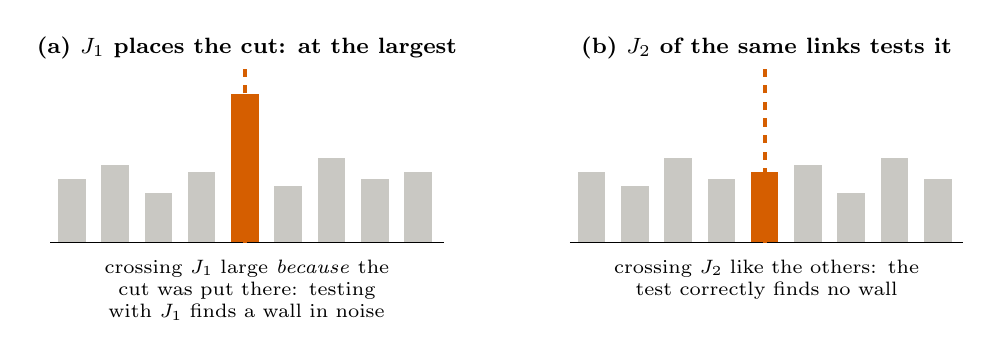
\begin{tikzpicture}[fig, yscale=0.9]
\def\jone{{0.9,1.1,0.7,1.0,2.1,0.8,1.2,0.9,1.0}}
\def\jtwo{{1.0,0.8,1.2,0.9,1.0,1.1,0.7,1.2,0.9}}
\begin{scope}
  \node[lab] at (2.5,2.75) {(a) $J_1$ places the cut: at the largest};
  \foreach \i in {0,...,8} {
    \pgfmathsetmacro{\h}{\jone[\i]}
    \ifnum\i=4 \def\col{cAcc}\else\def\col{cGrid}\fi
    \fill[\col] (0.55*\i+0.1,0) rectangle (0.55*\i+0.45,\h);
  }
  \draw (0,0) -- (5.0,0);
  \draw[wall, dashed] (2.475,0) -- (2.475,2.45);
  \node[small, text width=4.8cm, anchor=north] at (2.5,-0.1) {crossing $J_1$ large \emph{because} the cut was put there:
    testing with $J_1$ finds a wall in noise};
\end{scope}
\begin{scope}[shift={(6.6,0)}]
  \node[lab] at (2.5,2.75) {(b) $J_2$ of the same links tests it};
  \foreach \i in {0,...,8} {
    \pgfmathsetmacro{\h}{\jtwo[\i]}
    \ifnum\i=4 \def\col{cAcc}\else\def\col{cGrid}\fi
    \fill[\col] (0.55*\i+0.1,0) rectangle (0.55*\i+0.45,\h);
  }
  \draw (0,0) -- (5.0,0);
  \draw[wall, dashed] (2.475,0) -- (2.475,2.45);
  \node[small, text width=4.8cm, anchor=north] at (2.5,-0.1) {crossing $J_2$ like the others:
    the test correctly finds no wall};
\end{scope}
\end{tikzpicture}

\caption{Selection bias, schematic. Left: on a chain without a wall the cut is put at the
largest noisy $J_1$. Right: the independent $J_2$ of the same link is ordinary.}\label{fig:selection}
\end{figure}

\begin{tech}
The spectral cut always proposes a split, even inside a single phase. It is kept as a wall
only if its crossing links jump more than the inner links, measured with $J_2$, which did not
take part in placing it. Let $x_i=\log J_2$ on the $n_1$ crossing links and $y_j=\log J_2$ on the $n_2$ inner links
of the region. The Mann-Whitney statistic
\[
U=\sum_{i,j}\Big[\mathbf 1(x_i>y_j)+\tfrac12\,\mathbf 1(x_i=y_j)\Big],\qquad
\mathrm{AUC}=U/(n_1n_2),
\]
is the number of (crossing, inner) pairs in which the crossing link jumps more; its one-sided
$p$-value tests whether crossing jumps are stochastically larger. The cut is a wall if
$p<\alpha=10^{-3}$ \emph{and} the ratio of medians $e^{\med x-\med y}\ge1.5$ (\code{RATIO}):
the first condition says the difference is not noise, the second that it is large enough to
matter. Neighbouring links share points, so they are not independent: $p$ is used as a
score with a strict threshold, not as an exact probability.

\emph{Selection bias.} If the cut were tested with $J_1$, the one that placed it, the test
would be conditioned on its own outcome (Fig.~\ref{fig:selection}); on pure noise it finds walls in more than half of the tables (Fig.~\ref{fig:selectiondata}). This is the ``look-elsewhere'' problem of particle
physics, or judging a peak's height on the same noisy spectrum used to locate it. Splitting
the sample (one half to select, the other to test) removes it, at the price of power: each
test uses half of the runs. On the demo, five cuts are tried and two are kept (Figs.~\ref{fig:testsdata}
and~\ref{fig:cuttree}).
\end{tech}

\begin{figure}[H]
\centering
\includegraphics[width=0.85\textwidth]{data/selection.pdf}
\caption{The first cut on 40 synthetic tables of pure noise ($10\times8$ points, 2 runs of 5
snapshots, 6 descriptors). Tested with $J_1$, it passes both conditions (and would be a wall)
in 24 of 40 tables; tested with $J_2$, in 0 of 40. On 60 synthetic tables (noise, smooth
drifts, two and three phases), the count of phases was wrong in 41 tables with $J_1$ and
right in all 60 with $J_2$.}\label{fig:selectiondata}
\end{figure}

\begin{figure}[H]
\centering
\includegraphics[width=0.85\textwidth]{data/tests.pdf}
\caption{All five cuts tried on the demo: $\log_{10}J_2$ of the inner links (grey) and of the
crossing links, with medians (bars). Cuts 1 (uniform against patterned) and 2 (hexagons
against stripes) are walls; cuts 3 to 5, inside each phase, are not. Many jumps sit at the
floor (bottom).}\label{fig:testsdata}
\end{figure}

\begin{figure}[H]
\centering
% The recursion of cuts on the demo (numbers from docs/documentation/data/numbers.txt).
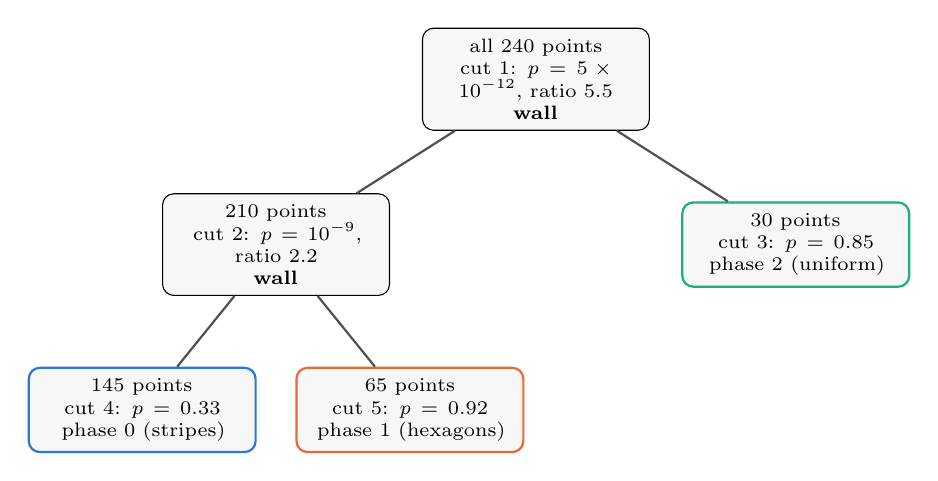
\begin{tikzpicture}[fig, level distance=2.1cm,
  every node/.style={blk, text width=2.6cm, font=\scriptsize},
  level 1/.style={sibling distance=6.6cm}, level 2/.style={sibling distance=3.4cm},
  edge from parent/.style={draw, thick, cInk2}]
\node {all 240 points\\ cut 1: $p=5\times10^{-12}$, ratio 5.5\\ \textbf{wall}}
  child {node {210 points\\ cut 2: $p=10^{-9}$, ratio 2.2\\ \textbf{wall}}
    child {node[draw=cP0, thick] {145 points\\ cut 4: $p=0.33$\\ phase 0 (stripes)}}
    child {node[draw=cP1, thick] {65 points\\ cut 5: $p=0.92$\\ phase 1 (hexagons)}}}
  child {node[draw=cP2, thick] {30 points\\ cut 3: $p=0.85$\\ phase 2 (uniform)}};
\end{tikzpicture}

\caption{The recursion on the demo: two walls, three phases. Cut 3 is inside the uniform
region (all its jumps at the floor), cuts 4 and 5 inside stripes and hexagons.}\label{fig:cuttree}
\end{figure}

\begin{codebox}
\textbf{Files.} \srcref{src/phasewall/walls.py}: \code{test_cut}
(\code{scipy.stats.mannwhitneyu}, \code{alternative="greater"}), \code{split_regions(...,
log_test=...)}, \code{find_walls} (everything), \code{phases_against_ratio} (robustness).
Tables of the result: \code{nodes} (parameters, runs, snapshots, spread, mixed, region,
phase), \code{edges} (\code{jump}, \code{jump_select} $=J_1$, \code{jump_test} $=J_2$,
contrast, wall), \code{cuts} (every cut tried).

\textbf{Tests.} No wall in pure noise (5 seeds) or under a smooth drift; exactly the 8 links
between $a=5$ and $a=6$ for two phases; the right 12 links for three phases on a smooth
background; the count against \code{RATIO} is 2, 2, 1 for ratios 1.5, 2, $10^6$.
\end{codebox}

%======================================================================
\section{Mixed points}\label{sec:mixed}
%======================================================================

\begin{tech}
Next to some transitions, runs at the same parameters end in different states depending on
their random start; the two halves of such a point differ far more than those of an ordinary
point, an independent sign of a boundary. For each point the unclipped statistic $E_a=D^2(a_1,a_2)$ is compared with all points:
$z_a=(E_a-\med E)/\max(1.4826\,\mathrm{MAD}(E),\,\text{floor}^2)$, and the point is mixed if
$z_a>6$ (\code{MIXED_K}). The unclipped value scatters around 0 for an ordinary point, so the
median and the median absolute deviation are meaningful (with clipped values half of them
were 0 and almost every point was flagged). The threshold is high because $E$ is
right-skewed: on pure noise, ordinary points reach $z=5$ to 6.

\emph{Physics parallel.} A first-order transition has a range of coexistence between two
spinodals, where both states are locally stable and the one reached depends on the history
(hysteresis). Runs from random initial conditions then split between two states, and the
distribution of their descriptors is bimodal.
\end{tech}

\begin{figure}[H]
\centering
\includegraphics[width=0.48\textwidth]{data/mixed.pdf}
\caption{The demo: no point above the threshold. With runs to $t=500$ only, one point,
$(\varepsilon,g)=(0.125,0.2)$, was above it: its runs were still changing (a transient, not a
bistable point).}
\end{figure}

\begin{codebox}
\textbf{Files.} \srcref{src/phasewall/walls.py}: \code{robust_outliers}, column \code{mixed}
of \code{nodes}. \textbf{Test:} on a flat table where one of the two runs of one point is in
another state, that point and only that point is flagged.
\end{codebox}

%======================================================================
\section{The demo: the Swift-Hohenberg equation}\label{sec:demo}
%======================================================================

\begin{tech}
\[
\partial_tu=\varepsilon u-(1+\nabla^2)^2u+gu^2-u^3 .
\]
\textbf{Linear stability.} For $u\propto e^{i\mathbf k\cdot\mathbf r+\sigma t}$,
$\sigma(k)=\varepsilon-(1-k^2)^2$ (Fig.~\ref{fig:sh}a): the uniform state is stable for
$\varepsilon<0$, and for $\varepsilon>0$ a band of wavenumbers around $k=1$ grows. Near
$\varepsilon=0$ the relaxation time $1/|\varepsilon|$ diverges (critical slowing down), which
is why the demo grid avoids $\varepsilon=0$ ($\varepsilon=-0.075,-0.025,0.025,\dots$).

\textbf{Amplitude equations.} With $u=\sum_{j=1}^3A_je^{i\mathbf k_j\cdot\mathbf r}+\text{c.c.}$,
$|\mathbf k_j|=1$, $\mathbf k_1+\mathbf k_2+\mathbf k_3=0$, projecting the equation on
$e^{i\mathbf k_1\cdot\mathbf r}$ gives
\[
\dot A_1=\varepsilon A_1+2g\,\bar A_2\bar A_3-3|A_1|^2A_1-6\big(|A_2|^2+|A_3|^2\big)A_1
\]
(the quadratic term couples the resonant triad: $-\mathbf k_2-\mathbf k_3=\mathbf k_1$).
Stripes ($A_1=A$, $A_2=A_3=0$): $A^2=\varepsilon/3$, so $u=2A\cos x$ and
$\std u=\sqrt{2\varepsilon/3}$, which the demo reproduces (Fig.~\ref{fig:amplitude}).
Hexagons ($A_j=R$): $\varepsilon+2gR-15R^2=0$, $R_\pm=(g\pm\sqrt{g^2+15\varepsilon})/15$,
$\std u=\sqrt6\,R$. In the standard form $\dot A=\mu A+\nu\bar A\bar A-|A|^2A-G(\ldots)A$
($\mu=\varepsilon/3$, $\nu=2g/3$, $G=2$), the known thresholds give
\begin{align*}
\varepsilon_A&=-\tfrac{g^2}{15} &&\text{(hexagons appear)},\\
\varepsilon_R&=\tfrac43g^2 &&\text{(stripes become stable)},\\
\varepsilon_H&=\tfrac{16}3g^2 &&\text{(hexagons become unstable)}.
\end{align*}
Hexagons bifurcate subcritically, and stripes and hexagons are both stable between
$\varepsilon_R$ and $\varepsilon_H$ (Fig.~\ref{fig:sh}b). These results hold for small
$\varepsilon$ and $g$ (formally $g=O(\sqrt\varepsilon)$).

\textbf{Numerics.} Periodic box of $64\times64$ points holding 8 wavelengths $2\pi$
($\Delta x=0.785$), pseudo-spectral, semi-implicit with a stabilising constant $C=2$:
\[
\big[1-\Delta t(\varepsilon-(1-k^2)^2-C)\big]\hat u^{n+1}=\hat u^n+\Delta t\,\mathcal F\!\left[gu^2-u^3+Cu\right]^n,
\qquad\Delta t=0.25 .
\]
Each run starts from noise of amplitude 0.1; snapshots are saved every 25 time units from
$t=5000$ (6 snapshots; see the steady-state check below). Grid: $\varepsilon\in[-0.075,0.675]$ step 0.05 (16 values),
$g\in[0,1.4]$ step 0.1 (15), 8 seeds per point: 1920 runs. A reference label per run, used only
to check \pw{}: uniform if $\std u<10^{-3}$, hexagons if $|\text{skewness}|>0.4$, else stripes.
\end{tech}

\begin{figure}[H]
\centering
% Swift-Hohenberg: (a) linear growth rate; (b) weakly nonlinear branches for g = 0.25.
% Coordinates in cm: (a) x = 2.5 k, y = 5 sigma; (b) x = 12 eps, y = 5 std(u).
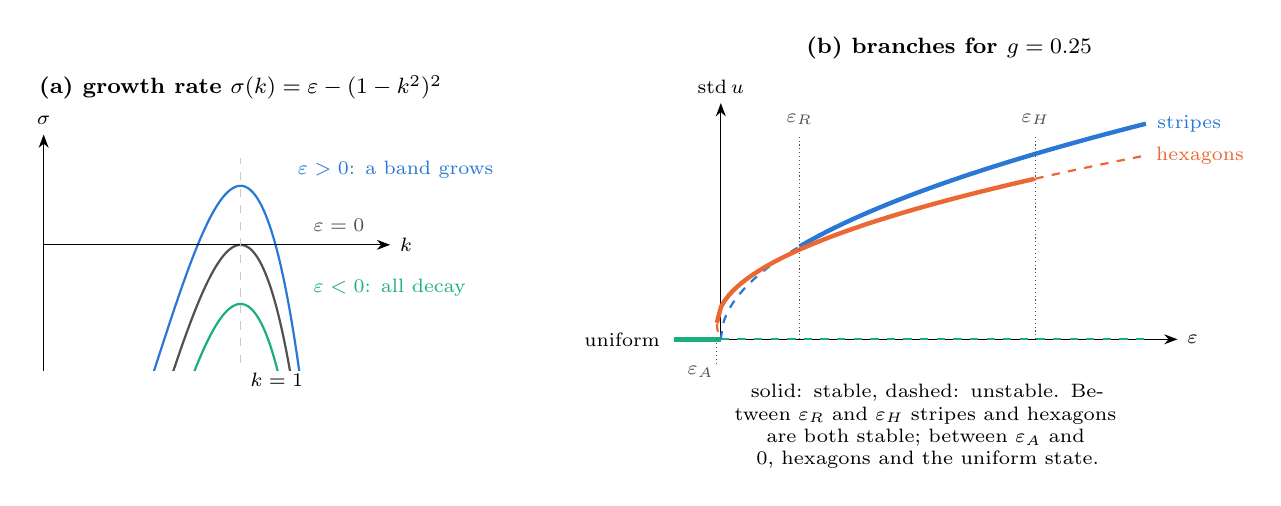
\begin{tikzpicture}[fig]
\begin{scope}
  \node[lab] at (2.5,2.0) {(a) growth rate $\sigma(k)=\varepsilon-(1-k^2)^2$};
  \begin{scope}
    \clip (0,-1.6) rectangle (4.2,1.4);
    \foreach \e/\c in {0.15/cP0, 0/cInk2, -0.15/cP2}
      \draw[\c, thick, domain=0.3:1.6, samples=80, smooth] plot ({2.5*\x}, {5*(\e-(1-\x*\x)^2)});
  \end{scope}
  \draw[->] (0,0) -- (4.4,0) node[right, small] {$k$};
  \draw[->] (0,-1.6) -- (0,1.4) node[above, small] {$\sigma$};
  \draw[dashed, cGrid] (2.5,-1.5) -- (2.5,1.1);
  \node[small, anchor=north west] at (2.5,-1.5) {$k=1$};
  \node[small, cP0, anchor=west] at (3.1,0.95) {$\varepsilon>0$: a band grows};
  \node[small, cInk2, anchor=west] at (3.3,0.25) {$\varepsilon=0$};
  \node[small, cP2, anchor=west] at (3.3,-0.55) {$\varepsilon<0$: all decay};
\end{scope}
\begin{scope}[shift={(8.6,-1.2)}]
  % g = 0.25: eps_A = -0.0042, eps_R = 0.0833, eps_H = 0.333
  \node[lab] at (2.9,3.7) {(b) branches for $g=0.25$};
  \draw[->] (-0.6,0) -- (5.8,0) node[right, small] {$\varepsilon$};
  \draw[->] (0,0) -- (0,3.0) node[above, small] {$\std u$};
  \draw[cP2, line width=1.6pt] (-0.6,0) -- (0,0);
  \draw[cP2, thick, dashed] (0,0) -- (5.4,0);
  \draw[cP0, thick, dashed, domain=0:0.0833, samples=40] plot ({12*\x}, {5*sqrt(2*\x/3)});
  \draw[cP0, line width=1.6pt, domain=0.0833:0.45, samples=40] plot ({12*\x}, {5*sqrt(2*\x/3)})
    node[right, small] {stripes};
  \draw[cP1, line width=1.6pt, domain=-0.00416:0.333, samples=80] plot ({12*\x}, {5*sqrt(6)*(0.25+sqrt(0.0625+15*\x))/15});
  \draw[cP1, thick, dashed, domain=0.333:0.45, samples=20] plot ({12*\x}, {5*sqrt(6)*(0.25+sqrt(0.0625+15*\x))/15})
    node[right, small] {hexagons};
  \draw[cP1, thick, dashed, domain=-0.00416:0, samples=30] plot ({12*\x}, {5*sqrt(6)*(0.25-sqrt(0.0625+15*\x))/15});
  \draw[cInk2, densely dotted] (12*0.0833,0) -- (12*0.0833,2.6) node[above, small] {$\varepsilon_R$};
  \draw[cInk2, densely dotted] (12*0.333,0) -- (12*0.333,2.6) node[above, small] {$\varepsilon_H$};
  \draw[cInk2, densely dotted] (-0.05,0) -- (-0.05,-0.3) node[below left, small, inner sep=1pt] {$\varepsilon_A$};
  \node[small, anchor=east] at (-0.65,0) {uniform};
  \node[small, text width=5.6cm, anchor=north] at (2.6,-0.45) {solid: stable, dashed: unstable.
    Between $\varepsilon_R$ and $\varepsilon_H$ stripes and hexagons are both stable;
    between $\varepsilon_A$ and 0, hexagons and the uniform state.};
\end{scope}
\end{tikzpicture}

\caption{(a) Linear growth rate. (b) Weakly nonlinear branches for $g=0.25$ (formulas
above).}\label{fig:sh}
\end{figure}

\begin{figure}[H]
\centering
\includegraphics[width=0.5\textwidth]{data/amplitude.pdf}
\caption{Standard deviation of $u$ at $g=0$ in the demo against $\sqrt{2\varepsilon/3}$: within 1\%
up to $\varepsilon=0.3$, 3\% below it at $\varepsilon=0.675$, where the weakly nonlinear theory no
longer holds exactly.}\label{fig:amplitude}
\end{figure}

\subsection{Result}

\begin{figure}[H]
\centering
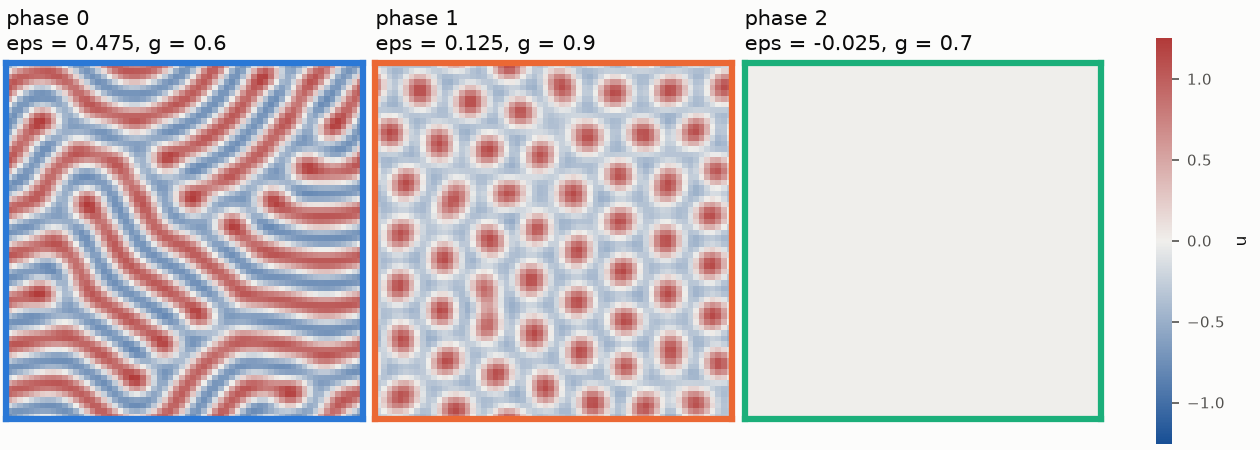
\includegraphics[width=0.85\textwidth]{../figures/snapshots.png}
\caption{One snapshot from the central point of each phase found, on one colour scale.}
\end{figure}

\begin{figure}[H]
\centering
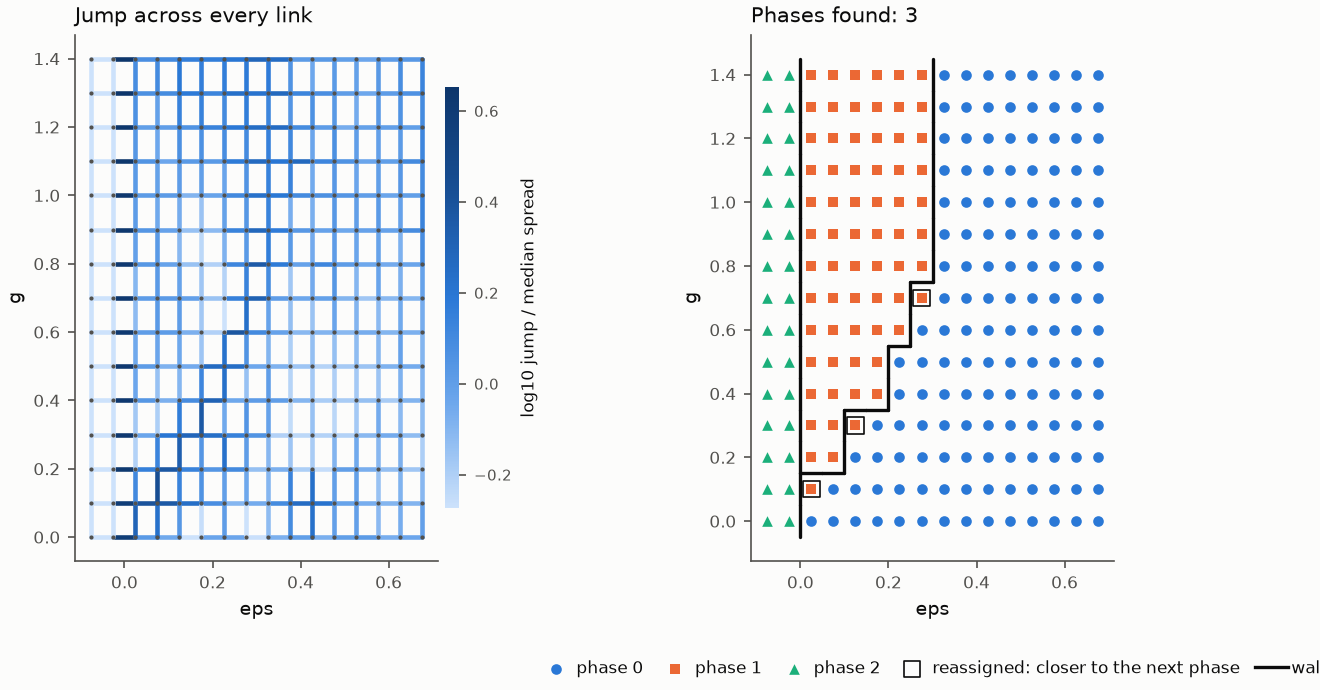
\includegraphics[width=\textwidth]{../figures/phase_map.png}
\caption{Left: $J/s$ on every link (log scale). Middle: the phases found, the walls (black)
and the mixed point (ring). Right: reference labels, never seen by \pw{}.}\label{fig:phasemap}
\end{figure}

\begin{tech}
\textbf{Agreement} (Fig.~\ref{fig:phasemap}). 3 phases; 235 of 240 points carry the most common
reference label of their region. Uniform: 30 of 30; hexagons: 64 of 64; phase 0 holds 141 stripe
points and 5 hexagon points. These 5 lie on the hexagon-stripe boundary ($(0.025,0.1)$,
$(0.275,0.7)$ and $\varepsilon=0.325$ for $g=1.0$ to 1.2): at each of them the 8 runs split
between hexagons (5 or 6 runs) and stripes (2 or 3), so the boundary passes through these points
and either side is a fair answer. The mixed flag fires at no point: a split of 6 to 2 between
runs that are themselves mixed is not enough to stand out.

\textbf{Steady state and pinned mixed states.} With runs to $t=500$ (the first version of the
demo) 9 boundary points disagreed with the reference. Their 72 runs were continued to
$t=2500$, 5000 and $20\,000$: only one point changed (3 of its runs turned from hexagons to stripes
before $t=5000$), hence the run time of $5000$. At $t=20\,000$ every run is frozen (its pattern
changes by less than $10^{-5}$ over 500 time units), and many still hold patches of spots and
stripes side by side: the fronts between the two states are pinned to the pattern, a known
effect of patterns in a gradient flow (the front would move if it did not lock to the
underlying lattice). Such runs are steady mixed states, not transients; at $(0.125,0.3)$ four
runs end as perfect stripes and four as perfect hexagons, a bistable point as the amplitude
equations predict ($\varepsilon_R=0.12<0.125<\varepsilon_H=0.48$ at $g=0.3$).

\textbf{Against the theory.} At small $g$ the found boundary lies between $\varepsilon_R$ and
$\varepsilon_H$ as it should for runs from random starts (for $g=0.2$:
$\varepsilon_R=0.053$, $\varepsilon_H=0.21$, boundary between 0.075 and 0.125). At larger $g$
the found boundary saturates near $\varepsilon\approx0.3$, far below $\varepsilon_H$: the
amplitude equations are no longer valid there.

\textbf{A bistable region the demo cannot see.} For $\varepsilon_A<\varepsilon<0$ hexagons
coexist with the stable uniform state. Started from hexagons ($R=0.15$), runs at
$\varepsilon=-0.025$ stay hexagonal for $g=0.7$, 1.0 and 1.4 and decay for $g=0.5$, as
$\varepsilon_A=-g^2/15$ predicts (at $g\ge1$ hexagons also survive below $\varepsilon_A$, beyond
the validity of the theory). All demo runs start from small noise and end uniform there, so
\pw{} and the reference labels both see a single uniform phase: the method finds the
states the runs reach, not every stable state.

\textbf{Robustness.} The count is 3 for \code{RATIO} from 1.2 to 2.0 and 2 from 2.5 (the
uniform wall is the strongest). With only 2 runs per point the unbiased test misses the
hexagon-stripe wall ($p=0.04$); it is found from 6 runs per point on, which is why the demo
uses 8 (measured with the earlier runs to $t=500$).
\end{tech}

\begin{figure}[H]
\centering
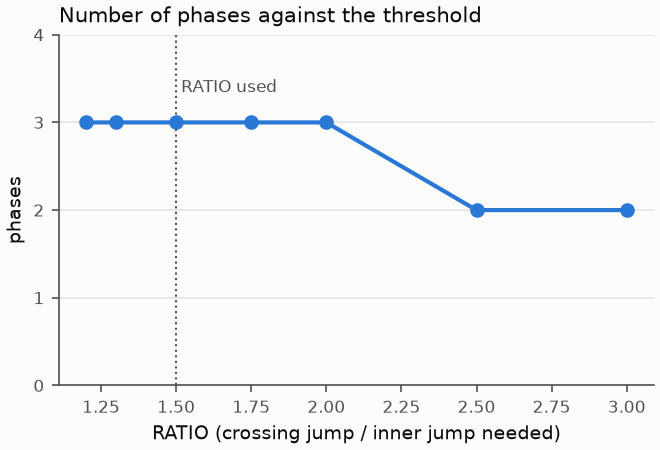
\includegraphics[width=0.45\textwidth]{../figures/robustness.png}
\caption{Number of phases against \code{RATIO}.}
\end{figure}

\begin{codebox}
\textbf{Files.} \srcref{src/phasewall/toy.py} (\code{simulate}, \code{reference_label},
\code{make_ensemble}), \srcref{src/phasewall/cli.py} (\code{phasewall demo}),
\srcref{src/phasewall/report.py}; tests \srcref{tests/test_toy.py}, \srcref{tests/test_cli.py}.
\code{phasewall demo data/demo --workers 8} writes the runs, \code{descriptors.csv} and
\code{walls/} (\code{summary.md}, tables, figures) in about eight minutes.
\textbf{Tests.} Six $(\varepsilon,g)$ points end in the expected state; the stripe amplitude is
$\sqrt{2\varepsilon/3}$ within 2\% at $\varepsilon=0.1$ and 0.2; the ensemble written by
\code{make_ensemble} is read back and described.
\end{codebox}

\subsection{Hand-made against learned description}\label{sec:comparison}

\begin{tech}
\textbf{Set-up} (\srcref{scripts/compare_describers.py}). The demo is described twice: as the
whole periodic box, and as a centred crop of $40\times40$ points (5 wavelengths) described
as a non-periodic frame (Sec.~\ref{sec:frames}). In each case four describers use the same rows
(the 5 snapshots of each run that have a partner $\Delta t$ earlier): the hand-made $f$, the
learned $f$ trained with seeds 0 and 1 (40 epochs, about 2 min on a laptop GPU), and the same
network with its random initial weights (untrained), which shows what the architecture gives
before any training. Walls use the default settings. Besides the phases and the agreement with
the reference labels, three numbers explain the result: the AUC of $J$ at true boundaries
(probability that a link between two reference states jumps more than a link inside one
state), the relative jump (median $J$ of a kind of link over the median of all jumps), and a
linear probe (ridge classifier of hexagons against stripes per snapshot, tested on held-out
parameter points; balanced accuracy).
\end{tech}

\begin{table}[H]
\centering\small
\begin{tabular}{@{}llcccccc@{}}
\toprule
frame & description & phases & agree & AUC & jump hex/stripes & jump uniform/pattern & probe \\
\midrule
periodic & hand-made & 3 & 235 & 0.98 & 1.92 & 4.41 & 1.00 \\
periodic & learned, seed 0 & 2 & 171 & 0.92 & 1.37 & 2.22 & 0.98 \\
periodic & learned, seed 1 & 2 & 171 & 0.89 & 1.30 & 2.13 & 0.98 \\
periodic & untrained & 2 & 171 & 0.80 & 1.18 & 1.91 & 0.95 \\
crop & hand-made & 3 & 235 & 0.99 & 2.04 & 5.00 & 0.99 \\
crop & learned, seed 0 & 2 & 171 & 0.88 & 1.17 & 2.25 & 0.96 \\
crop & learned, seed 1 & 2 & 171 & 0.82 & 1.08 & 2.27 & 0.94 \\
crop & untrained & 2 & 159 & 0.71 & 1.06 & 1.53 & 0.94 \\
\bottomrule
\end{tabular}
\caption{Comparison on the demo (agree: of 240 points; relative jumps about 1 inside a state:
0.96 to 1.00). Full table with walls, mixed points, robustness range, effective rank and
times: \href{\repo/blob/main/docs/comparison/summary.md}{\code{docs/comparison/summary.md}}.}\label{tab:comparison}
\end{table}

\begin{figure}[H]
\centering
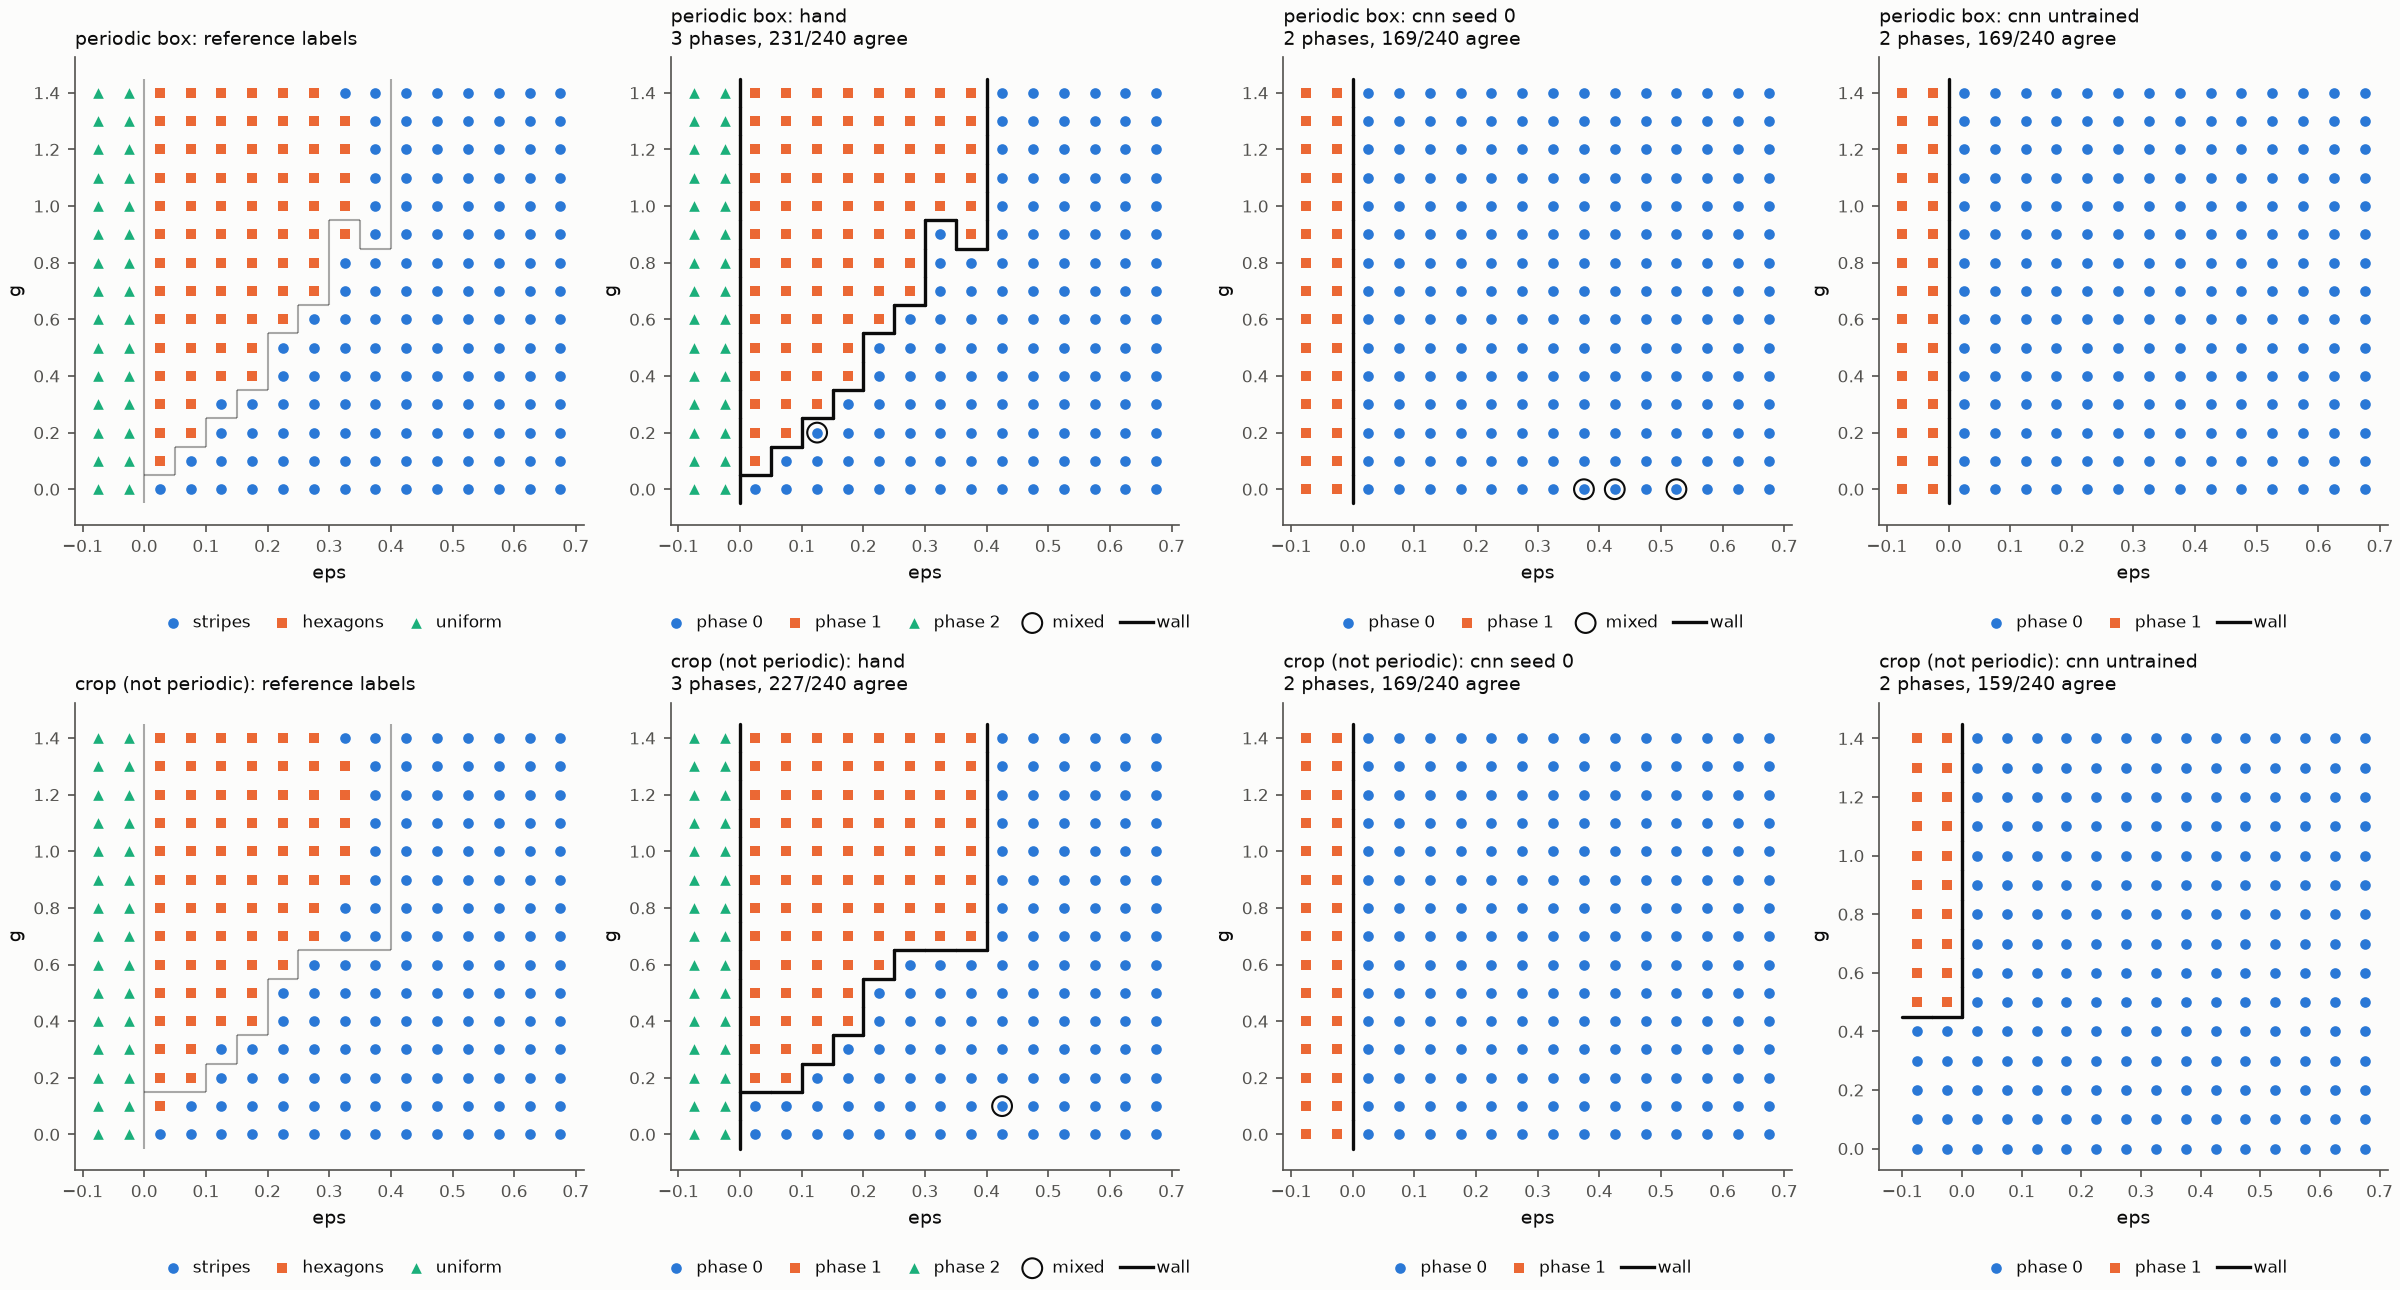
\includegraphics[width=\textwidth]{../comparison/phase_maps.png}
\caption{Reference labels and phases found by the hand-made description, the learned one
(seed 0) and the untrained network; top: periodic box, bottom: crop. Phases are coloured by
size (phase 0 is the largest), so colours do not name the same state in every panel.}\label{fig:comparisonmaps}
\end{figure}

\begin{figure}[H]
\centering
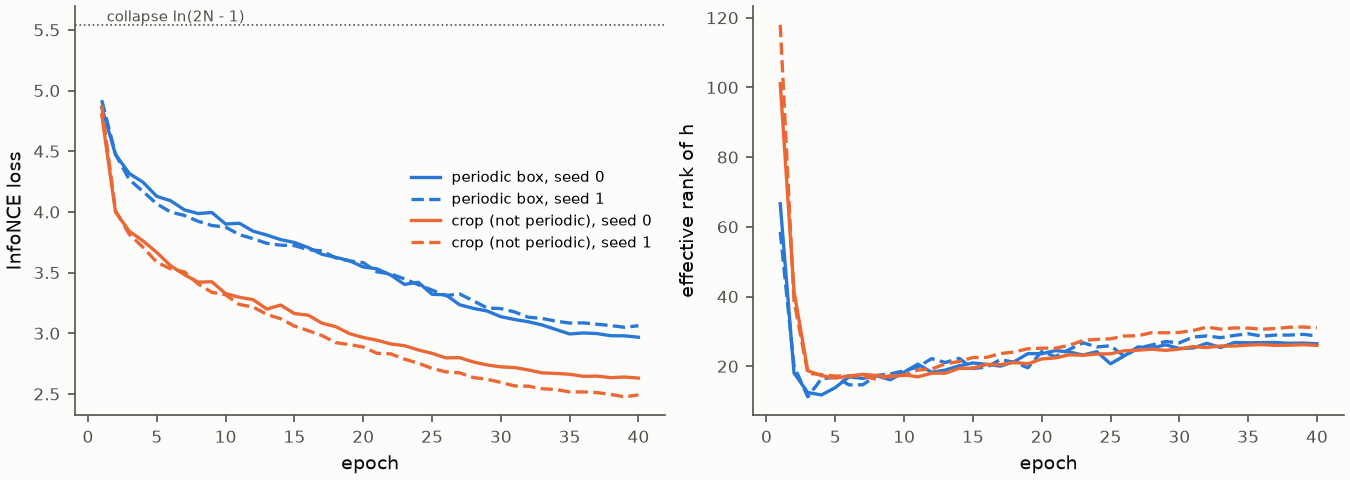
\includegraphics[width=0.85\textwidth]{../comparison/training.png}
\caption{Trainings: InfoNCE loss far below collapse ($\ln(2N-1)=5.54$) and effective rank of $h$
growing to 82--90 of 256 dimensions; alignment 0.999, uniformity $-3.35$ at the end.}\label{fig:training}
\end{figure}

\begin{tech}
\textbf{Result.} The hand-made description finds the three phases in both frames (235 of 240
points in each); every learned or untrained network finds two (uniform against patterned,
171 points). The trainings are healthy (Fig.~\ref{fig:training}), and the learned $h$ does
contain the difference between hexagons and stripes: the linear probe finds it in 94--98\% of
held-out points. What it lacks is a \emph{jump}: the median $J$ between a hexagon point and a
stripe point is 1.08--1.37 times the median of all jumps, little more than inside a phase,
against 1.9--2.0 for the hand-made description, whose skewness and domain counts change abruptly at that boundary.
The walls method looks for discontinuities, so a description that separates states along a
smooth direction is not enough. The spread within points is not the cause: in the periodic box
it is the same for both (27--29\% of the variance for the learned $h$, 30\% for the hand-made
$\mathbf x$); in the crop it is larger for the learned $h$ (48--52\% against 27\%).

\emph{Physics parallel.} The probe asks whether some combination of $h$ tells the two states
apart; the walls method needs a quantity that jumps between neighbouring points, as an order
parameter does at a first-order transition (the hexagon-stripe transition is one: it is
bistable). The learned $h$ behaves like a coordinate that varies smoothly through the
transition, while the hand-made descriptors include quantities that jump there (the skewness,
near 0 for stripes and finite for spots).

\textbf{More data does not help.} Trained on 2 or 4 runs per point instead of 8 (480 or 960
runs, the same number of training steps) and evaluated on all runs, the learned description
gives the same result: 2 phases, relative jump hexagons/stripes 1.01--1.07, probe 0.95--0.98
(measured with the earlier runs to $t=500$).

\textbf{To try.} The loss separates individual runs, so it is indifferent to whether two runs
differ within a phase or across a boundary. A combined table with the hand-made and the learned
columns as separate blocks (the walls method weights blocks equally) is compared with each
alone on every example (Sec.~\ref{sec:examples}). Positives from different runs of one parameter
point are another option, but they would hide bistable points.
\end{tech}

\subsection{Walls against blind grouping and a linear probe}\label{sec:methods}

\begin{tech}
\textbf{Question.} Is cutting the parameter graph better than grouping the runs by their
description alone, as in the blind search of hfml? Each description of the demo (hand-made,
learned seed 0 and 1, untrained) is given to the walls and to three blind methods
(\srcref{src/phasewall/baselines.py}, adapted from hfml): each run is the mean of its snapshots
(block-weighted as in Sec.~\ref{sec:compare}), compressed to the principal components that
explain 95\% of the variance, then
\begin{itemize}[leftmargin=1.2em, itemsep=1pt]
\item \emph{Gaussian mixture}: $p(\mathbf x)=\sum_{j=1}^k\pi_j\,\mathcal N(\mathbf x;\boldsymbol\mu_j,\Sigma_j)$,
  fitted by expectation-maximisation for $k=1\ldots10$; $k$ is the one with the smallest
  $\mathrm{BIC}=-2\ln\hat L+p\ln n$ ($p$ parameters, $n$ runs), likelihood penalised by model size;
\item \emph{k-means}: minimises $\sum_i|\mathbf x_i-\boldsymbol\mu_{c(i)}|^2$ for $k=2\ldots10$; $k$ is
  the one with the largest mean silhouette $s_i=(b_i-a_i)/\max(a_i,b_i)$ ($a_i$: mean distance of
  run $i$ to its own group, $b_i$: to the nearest other group);
\item \emph{HDBSCAN}: groups are the regions of high density that persist over a range of density
  levels, with at least $m$ runs ($m=5,10,20,40$); runs in sparse regions are noise.
\end{itemize}
None of them knows the parameter grid. The label of a point is the most common group of its
runs. Scores: groups found; agreement (points carrying the most common reference label of
their group, as for the walls); the adjusted Rand index
$\mathrm{ARI}=(\mathrm{RI}-\mathbb E[\mathrm{RI}])/(\max\mathrm{RI}-\mathbb E[\mathrm{RI}])$ between groups and reference
labels of the points (1: identical partitions, about 0: chance), on the points that are placed
and, as ARI$_{\rm all}$, with HDBSCAN noise counted as one more group; and the number of
connected pieces of the groups on the parameter grid (3 for the reference).

\textbf{Probe.} A logistic regression $P(y=c\,|\,\mathbf x)=e^{\mathbf w_c\cdot\mathbf x+b_c}/\sum_{c'}e^{\mathbf w_{c'}\cdot\mathbf x+b_{c'}}$
of the three reference states from the description of each snapshot ($L_2$ penalty, $C=1$),
trained and tested in 5 folds of whole parameter points (GroupKFold: no point in the training
and the test of the same fold); balanced accuracy. It sees the labels: it is the best a linear
reading of the description can do, not a way to find the states.

\emph{Physics parallel.} Blind grouping looks for clusters in the space of descriptions, as one
looks for peaks in a histogram of an order parameter; the walls look for discontinuities along
the control parameters, as one locates a transition by scanning a parameter and watching for a
jump. The first needs the states to form separate clouds; the second needs only that the
description changes faster across a boundary than inside a phase, and gives regions that are
connected in parameter space by construction.
\end{tech}

\begin{table}[H]
\centering\small
\begin{tabular}{@{}lllcccccc@{}}
\toprule
frame & description & method & groups & agree & ARI & ARI$_{\rm all}$ & pieces & noise \\
\midrule
periodic & hand-made & walls & 3 & 235 & 0.93 & 0.93 & 3 & 0 \\
 & & mixture ($k=10$ by BIC) & 8 & 230 & 0.38 & 0.38 & 13 & 0 \\
 & & k-means ($k=7$ by silhouette) & 5 & 235 & 0.58 & 0.58 & 5 & 0 \\
 & & HDBSCAN, $m=10$ & 7 & 216 & 0.77 & 0.66 & 11 & 12\% \\
 & & HDBSCAN, $m=20$ & 6 & 205 & 0.78 & 0.59 & 10 & 20\% \\
\addlinespace
 & learned (seed 0) & walls & 2 & 171 & 0.36 & 0.36 & 2 & 0 \\
 & & mixture ($k=10$) & 10 & 191 & 0.14 & 0.14 & 18 & 0 \\
 & & k-means ($k=10$) & 10 & 182 & 0.11 & 0.11 & 24 & 0 \\
 & & HDBSCAN, $m=10$ & 2 & 171 & 0.36 & 0.36 & 2 & 2\% \\
\addlinespace
crop & hand-made & walls & 3 & 235 & 0.93 & 0.93 & 3 & 0 \\
 & & mixture ($k=10$) & 9 & 238 & 0.48 & 0.48 & 15 & 0 \\
 & & k-means ($k=2$) & 2 & 171 & 0.36 & 0.36 & 2 & 0 \\
 & & HDBSCAN, $m=20$ & 3 & 237 & 0.97 & 0.96 & 3 & 4\% \\
\addlinespace
 & learned (seed 0) & walls & 2 & 171 & 0.36 & 0.36 & 2 & 0 \\
 & & mixture ($k=10$) & 10 & 192 & 0.13 & 0.13 & 38 & 0 \\
 & & HDBSCAN, $m=10$ & 2 & 171 & 0.36 & 0.36 & 2 & 4\% \\
\bottomrule
\end{tabular}
\caption{Walls against blind grouping on the same descriptions (agree: of 240 points; noise:
share of runs that HDBSCAN cannot place). Every method, setting and description, with seed 1 and
the untrained network:
\href{\repo/blob/main/docs/comparison/summary.md}{\code{docs/comparison/summary.md}}.}\label{tab:methods}
\end{table}

\begin{figure}[H]
\centering
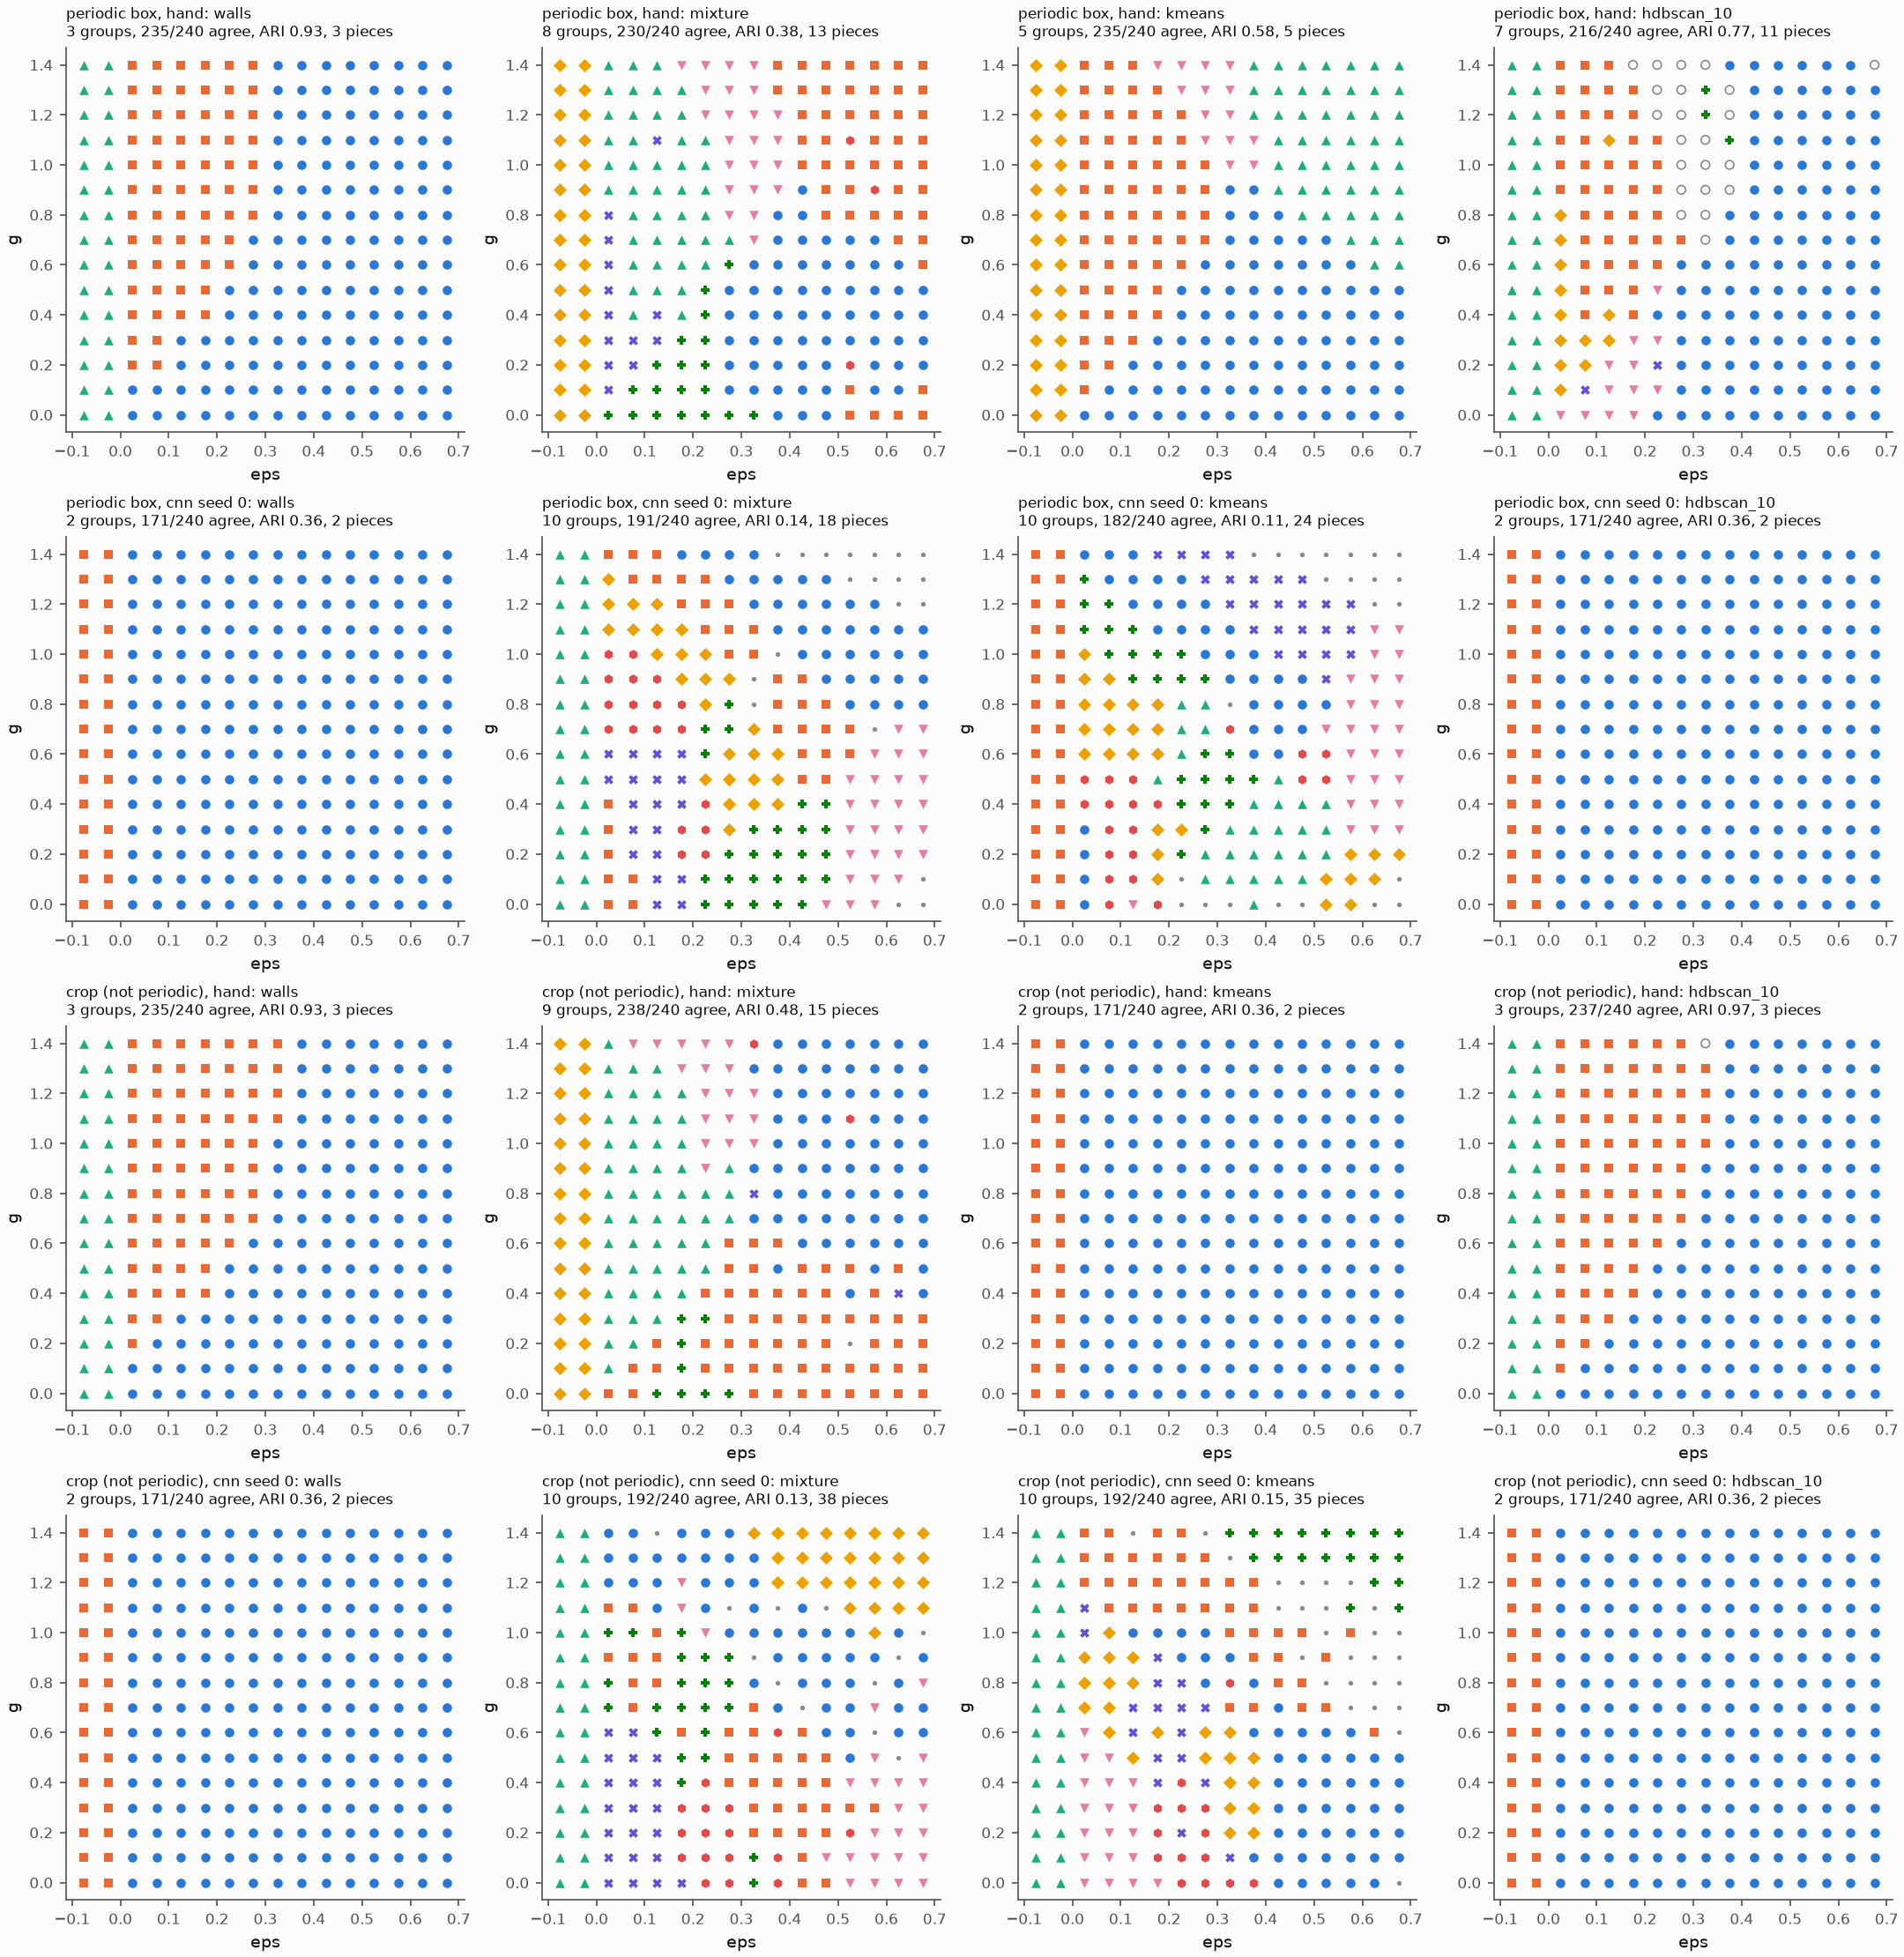
\includegraphics[width=\textwidth]{../comparison/methods_maps.png}
\caption{Majority group of every point for the walls, the mixture, k-means and HDBSCAN ($m=10$),
on the hand-made and the learned description, periodic box and crop. Groups are coloured by size;
open grey circles: points that HDBSCAN calls noise.}\label{fig:methodsmaps}
\end{figure}

\begin{tech}
\textbf{Result.} In the periodic box only the walls give the three states as three connected
regions (ARI 0.93). The mixture asks for the top of its range ($k=10$ by BIC, as in hfml) and
slices the phases into 13 to 15 pieces along the smooth drift of the description with
$\varepsilon$ and $g$; its high agreement (230 and 238) only reflects many small pure groups,
which ARI and the pieces expose. k-means chooses $k=7$ in the periodic box (5 groups on the
points) and $k=2$ in the crop (uniform against patterned). HDBSCAN leaves 12--20\% of the runs
as noise in the periodic box and breaks the uniform state into small groups; in the crop, with
sizes 10 and 20, it finds the three states (ARI 0.97 on the points it places, 0.96 with its 4\%
of noise), slightly closer to the reference than the walls (0.93). With the learned
description no method finds the hexagon-stripe boundary: the mixture and k-means cut the
patterned region into bands that follow $\varepsilon$ and $g$.

\textbf{Probe.} The logistic regression recognises the three states on held-out points with
balanced accuracy 0.999 and 0.995 (hand-made, periodic and crop), 0.960--0.981 (learned) and
0.954--0.958 (untrained). Every description contains the states; they differ in how the states
are laid out. Blind grouping needs separate clouds, which the descriptions have only in part
(in the periodic box the hexagon and stripe clouds touch and drift with the parameters; in the
crop they separate enough for HDBSCAN). The walls need only a
jump along the parameter grid, which the hand-made description has and the learned one lacks.
\end{tech}

\begin{codebox}
\textbf{Files.} \srcref{src/phasewall/baselines.py} (\code{run_matrix}, \code{reduce},
\code{fit_mixture}, \code{fit_kmeans}, \code{fit_hdbscan}, \code{blind_groups},
\code{point_scores}, \code{probe}; scikit-learn: \code{GaussianMixture}, \code{KMeans},
\code{HDBSCAN}, \code{LogisticRegression}, \code{GroupKFold}), extra \code{[baselines]};
\srcref{scripts/compare_describers.py} (\code{compare_methods}, \code{method_figure});
tests \srcref{tests/test_baselines.py}.

\textbf{Tests.} Three well separated clouds on a grid are found by the mixture, k-means and
HDBSCAN (3 groups, all points, ARI 1, 3 pieces); two separate states described alike give one
group in two pieces; the probe is above 0.95 for labels the description contains and near 0.5
for random labels; no ARI when every run is noise.
\end{codebox}

\subsection{An unsupervised threshold tree}\label{sec:tree}

\begin{tech}
\textbf{Idea.} A phase boundary often shows as a jump of one descriptor, an order parameter: the
amplitude at the uniform state, the skewness or the number of low domains between hexagons and
stripes. The tree looks for such a descriptor and a threshold, splits the parameter points of a
region in two, and repeats on each side. The leaves are the candidate phases, and each wall comes
with a rule that can be read. No label and no number of phases is given: supervised trees, fitted
to labels, are not part of \pw{}.

\textbf{Values.} Every descriptor is standardised over all snapshots; the value of a point is the
median over its snapshots, computed separately on the two halves of its runs ($v_1$ and $v_2$,
as for the walls, Sec.~\ref{sec:compare}).

\textbf{Splits} (on $v_1$). For a region $R$ and every descriptor, 32 candidate thresholds at
quantiles of the point values split $R$ into $S$ (above) and $S'$, both with at least
\code{MIN_PHASE} points. A candidate is scored by
\[
\eta^2=\frac{n_Sn_{S'}(m_S-m_{S'})^2}{n^2\,\mathrm{var}(v)},\qquad
\mathrm{Ncut}=\frac{\cut(S,S')}{\vol(S)}+\frac{\cut(S,S')}{\vol(S')},\qquad
\text{score}=\eta^2\left(1-\tfrac12\mathrm{Ncut}\right),
\]
with $\cut$ and $\vol$ counted on the grid links of $R$ (unit weights). $\eta^2$, the share of the
variance between the sides (Otsu's criterion), is close to 1 for two tight clouds and small for a
smooth drift; $\mathrm{Ncut}$ is small when the sides are two contiguous regions of the parameter
plane and large for scattered points. The threshold is chosen anew in every region.

\textbf{Test} (on $v_2$, which did not choose the split). Three conditions: (i) the values of the
points on the two sides differ (Mann-Whitney between the points, $p<$ \code{ALPHA}), which pure
noise fails; (ii) along each parameter, the median jump of the descriptor across the crossing
links is compared with its median jump across the inner links along the same parameter, and the
ratios, weighted by the number of crossing links, must average at least \code{RATIO}, which a
smooth drift fails; (iii) the threshold puts at least 90\% of the points on the same side. In (ii),
comparing along the same parameter matters: a straight cut through a drift crosses mostly links
along the steep direction while the inner links mix steep and flat ones, which made the drift of
the mean of $u$ along $\varepsilon$ pass as a jump in a first version. A Mann-Whitney test on the
link jumps, as for the walls, had too little power for one noisy descriptor and a wall of a few
links.

\emph{Physics parallel.} Choosing the descriptor and the threshold is choosing an order parameter
and the value that separates two phases (the middle of a bimodal distribution, as between the
liquid and gas densities at coexistence); the normalised cut is the length of the interface
between the two regions of the parameter plane relative to their sizes, an interfacial energy.
\end{tech}

\begin{figure}[H]
\centering
\includegraphics[width=\textwidth]{data/tree_sh.pdf}
\caption{The threshold tree on the demo, with the halves as planned and swapped, and the
reference labels.}\label{fig:treesh}
\end{figure}

\begin{tech}
\textbf{Result on the demo.} Both trees make the same first two splits:
\code{u.amp.log10var} $\le-12$ (the uniform state: no amplitude) and \code{u.topo.below-1}
above 0.022 or 0.025 per unit area (hexagons: many separate domains of low $u$, the gaps between
spots). With the halves swapped these are the only accepted splits: 3 phases, 237 of 240 points
agree with the reference, ARI 0.96 (walls: 0.93). With the halves as planned a third split,
\code{u.shape.k00} (power at the longest wavelengths), cuts off 9 stripe points next to the
hexagon-stripe boundary: 4 phases, 235 points, ARI 0.90. The two rules found without labels are
the physical criteria behind the reference labels (amplitude, and a spot-like topology where the
reference uses the skewness).

\textbf{Limit.} When a point holds a single run, its two halves are snapshots of the same run,
strongly correlated: condition (i) then no longer protects against splits that only sort runs,
and on such data the tree splits far too much. Stopping rules for that case (only the splits found
with both halves; a minimum $\eta^2$ and a maximum Ncut; fewer, coarser descriptors) are to try.
\end{tech}

\begin{codebox}
\textbf{Files.} \srcref{src/phasewall/trees.py} (\code{point_values}, \code{best_split},
\code{test_split}, \code{fit_tree}, \code{rules_text}, \code{components} for a learned
description, \code{Tree.as_walls} for the plots); tests \srcref{tests/test_trees.py}.

\textbf{Tests.} No split in pure noise, under a drift along both parameters, or under a strong
drift along one parameter; two phases: the jumping descriptor and a threshold between its two
levels; three phases: two nested rules on the two jumping descriptors; the same tree with the
halves swapped; principal components (the number kept, the variance explained).
\end{codebox}

%======================================================================
\section{Further examples}\label{sec:examples}
%======================================================================

\begin{tech}
Swift-Hohenberg is a gradient flow: all its patterns end frozen, it has one field and three
states. Four more models test what it cannot; each was given a pilot scan to choose its window
and run time, and is checked for steady state (a sample of runs continued to 2 and 4 times the
run time). All are run by \srcref{scripts/run_examples.py} with the hand-made, the learned and the
combined description and every method; results in \code{docs/examples/}.

\textbf{Gray-Scott} (Pearson 1993; $u$, $v$; $F$, $k$): two uniform states, spots, isolated spots,
holes, stripes and labyrinths, moving states. On the first grid (steps 0.005 and 0.0025) 5 phases
are found and 113 of 143 points agree; the uniform states and the moving region are found, but the
pattern band, one to three points wide, is merged with a uniform state. Rerun on a grid twice as
fine to $t=40\,000$ (3 of 143 points still changed between $t=20\,000$ and $60\,000$).

\textbf{FitzHugh-Nagumo} (Hagberg-Meron form $\partial_tu=u-u^3-v+\nabla^2u$,
$\partial_tv=\varepsilon(u-a_1v-a_0)+\delta\nabla^2v$, $a_1=2$, $a_0=0$; $\varepsilon$, $\delta$):
a symmetric bistable medium with stationary fronts, moving domains and front turbulence, uniform
states (up or down at random, equivalent by symmetry) and Turing labyrinths, rings and spots. With
$a_0=-0.1$ nothing moves (pilot).

\textbf{Barkley} ($\partial_tu=\nabla^2u+\varepsilon^{-1}u(1-u)(u-(v+b)/a)$, $\partial_tv=u-v$,
$\varepsilon=0.02$; $a$, $b$): rest, plane wave trains and spirals, counted by their tips (points
around which the phase of $(u,v)$ winds by $2\pi$; on a periodic box they come in pairs).
Barkley's semi-implicit reaction step keeps $u$ in $[0,1]$; plain forward Euler blows up.

\textbf{Localised Swift-Hohenberg} (cubic-quintic equation $\partial_tu=\varepsilon u-(1+\nabla^2)^2u
+bu^3-u^5$; $a=\varepsilon/b^2$ and $b$): stripe patches that stay localised in the pinning range of
homoclinic snaking (dissipative solitons), vanish below it or invade the box above. With the
quadratic-cubic equation of the demo the pinning range of hexagon patches was narrower than 0.005
in $\varepsilon$ (pilot at $g=1$), and a patch started at small amplitude decays whatever $\varepsilon$:
the patches start on the upper branch (amplitude 1.4).
\end{tech}

\subsection{Results}\label{sec:examples-results}

Table~\ref{tab:examples} gives, for every example, the walls on the hand-made, the learned
(seed 0; seed 1 gives the same phases) and the combined description, the blind method closest
to the reference labels, the probe, and the unsupervised tree of Sec.~\ref{sec:tree} on the
hand-made description. Every method uses its defaults; the reference labels are used only for
the scores. All numbers: \code{docs/examples/overview.md} and \code{trees.csv}.

\begin{table}[H]
\centering\small
\begin{tabular}{@{}>{\raggedright}p{2.6cm}lrrr>{\raggedright}p{4.0cm}r@{}}
\toprule
example (points $\times$ seeds) & description & phases & agree & ARI & closest blind method (ARI, pieces) & probe \\
\midrule
Swift-Hohenberg ($240\times8$) & hand-made & 3 & 235 & 0.93 & HDBSCAN 20 (0.78, 10) & 1.00 \\
                               & learned   & 2 & 171 & 0.36 & HDBSCAN 20 (0.37, 2) & 0.98 \\
                               & combined  & 2 & 171 & 0.36 & k-means (0.36, 2) & 1.00 \\
                               & tree      & 4 / 3 & 235 / 237 & 0.90 / 0.96 & & \\
\addlinespace
Gray-Scott ($525\times4$)      & hand-made & 10 & 482 & 0.80 & k-means, $k=7$ (0.99, 23) & 0.96 \\
                               & learned   & 1 & 207 & 0 & HDBSCAN 20 (0.86, 8; 32\% noise) & 0.92 \\
                               & combined  & 8 & 503 & 0.86 & HDBSCAN 20 (0.82, 30) & 0.97 \\
                               & tree      & 16 / 21 & 499 / 492 & 0.84 / 0.82 & & \\
\addlinespace
localised SH ($105\times4$)    & hand-made & 3 & 103 & 0.96 & HDBSCAN 10 (1.00, 3; 13\% noise) & 1.00 \\
                               & learned   & 1 & 51 & 0 & HDBSCAN 20 (1.00, 2; 41\% noise) & 1.00 \\
                               & combined  & 1 & 51 & 0 & HDBSCAN 10 (1.00, 4; 17\% noise) & 1.00 \\
                               & tree      & 3 / 3 & 104 / 104 & 0.98 / 0.98 & & \\
\addlinespace
FitzHugh-Nagumo ($99\times4$)  & hand-made & 1 & 33 & 0 & HDBSCAN 20 (0.71, 16; 23\% noise) & 0.77 \\
                               & learned   & 1 & 33 & 0 & HDBSCAN 10 (0.71, 15; 35\% noise) & 0.70 \\
                               & combined  & 1 & 33 & 0 & HDBSCAN 20 (0.74, 16; 20\% noise) & 0.79 \\
                               & tree      & 1 / 1 & 33 / 33 & 0 / 0 & & \\
\addlinespace
Barkley ($165\times4$)         & hand-made & 2 & 132 & 0.59 & HDBSCAN 20 (0.84, 20; 14\% noise) & 0.99 \\
                               & learned   & 1 & 90 & 0 & HDBSCAN 10 (0.96, 6; 25\% noise) & 0.96 \\
                               & combined  & 2 & 132 & 0.59 & HDBSCAN 20 (0.86, 13; 21\% noise) & 0.99 \\
                               & tree      & 2 / 2 & 132 / 131 & 0.58 / 0.58 & & \\
\bottomrule
\end{tabular}
\caption{The examples. Agree: points whose phase carries their most common reference label;
ARI: adjusted Rand index with the reference labels of the points (noise left out for HDBSCAN);
pieces: connected pieces of the groups on the grid (the reference labels form 3 pieces for
Swift-Hohenberg and localised SH, 20 for Gray-Scott, whose boundaries are ragged); probe:
balanced accuracy of a logistic regression of the labels on held-out points (a ceiling, it sees
the labels). Tree: halves as given / swapped.}
\label{tab:examples}
\end{table}

\textbf{Steady state.} In Swift-Hohenberg and localised SH, the label of none of the 24 continued
runs changed, and the field changed by less than $10^{-4}$. In Gray-Scott the label of 2 to 3 of 24 runs changed, mostly with a field that
barely moved (the reference labeller near its thresholds between holes, stripes and spots), but
two runs next to the moving region started to move after $t=40\,000$. In FitzHugh-Nagumo no label
changed; the moving states keep moving, as they should. In Barkley, at $t=500$, 6 of 24 runs
went from spirals to plane waves by $t=2000$ (spiral pairs annihilate slowly), so Barkley was
rerun to $t=4000$; then no label of the 24 continued runs changed up to $t=16\,000$.

\textbf{One state per point: the walls and the tree work.} With the hand-made description, the
walls agree with the reference on 92 to 98\% of the points of Swift-Hohenberg, Gray-Scott and
localised SH (Fig.~\ref{fig:examples}). In Gray-Scott the ten phases follow the reference regions:
the two uniform states, the moving region, stripes, spots and isolated spots; the uniform state
lies in two places and counts as two phases. Most of the stripe band is flagged as mixed, although
only 19 of the 525 points have runs that end with different labels: the flag reflects the spread
of labyrinths there, not coexisting states. The tree reads its phases as rules: in localised SH,
\code{u.amp.log10var} alone (flat, small for a patch, large for stripes everywhere); in
Gray-Scott, flat or not, then moving or not (\code{u.dyn.moving}), then the shape of $S(k)$. It
over-splits Gray-Scott (16 and 21 leaves, 13 to 18 points in leaves below \code{MIN_PHASE}).

\textbf{Blind grouping is sometimes closer.} On Gray-Scott, k-means with $k=7$ matches the reference
labels better than the walls (ARI 0.99 against 0.80); its 23 pieces are close to the 20 of the
reference itself. On localised SH, HDBSCAN finds the three states exactly but leaves 13 to 41\% of
the runs as noise. Only on Swift-Hohenberg, where the hexagon and stripe clouds touch and drift,
are the walls clearly ahead.

\textbf{The learned description has no jump.} Alone, it gives one phase on Gray-Scott, localised SH,
FitzHugh-Nagumo and Barkley, and two on Swift-Hohenberg, while the probe still recognises the states (0.70
to 1.00): as on the demo (Sec.~\ref{sec:comparison}), the states are in $h$ but $h$ changes smoothly
across their boundaries. Combined with the hand-made description it helps on Gray-Scott (ARI 0.80
to 0.86) and removes walls on Swift-Hohenberg and localised SH, where the walls of the combined
table follow those of the learned one. Why the learned block dominates although it is weighted as
one block among the hand-made ones has not been looked into yet.

\textbf{Barkley: rest against activity only.} The walls and the tree find one wall, between
rest and the active states, within one grid step of the reference; plane waves and spirals form
one phase (ARI 0.59). At 52 of the 165 points the four runs do not end in the same state (26
points rest and spirals, 22 plane waves and spirals, 4 rest and plane waves): whether a spiral
pair survives depends on the initial condition. This is the second cause of the failure on
FitzHugh-Nagumo below. HDBSCAN on the learned description separates the three states best
(ARI 0.96) but leaves a quarter of the runs as noise.

\textbf{FitzHugh-Nagumo: the method's assumptions fail.} No method finds the states well (walls: one
phase; best ARI 0.74 with 20\% noise; probe below 0.8). Two causes were measured. (i) The model is
symmetric under $(u,v)\to(-u,-v)$ at $a_0=0$, but the description is not: the uniform runs end at
$u\approx-0.71$ (79 runs) or $+0.71$ (55), at random, and 22 points have both, which
\code{u.mom.mean} and \code{u.mom.skew} see as two states. (ii) 48 of the 99 points have runs
that end in different states (bistability between uniform states, fronts, patterns and motion).
The walls assume one state per point: here the spread of a point is as large as the jumps between
points (the first cut has crossing jumps 0.86 times the inner ones). A field rule for odd fields
(descriptors made even in $u$) would remove (i); (ii) needs a description of each point as a
mixture of states rather than one state.

\begin{figure}[H]
\centering
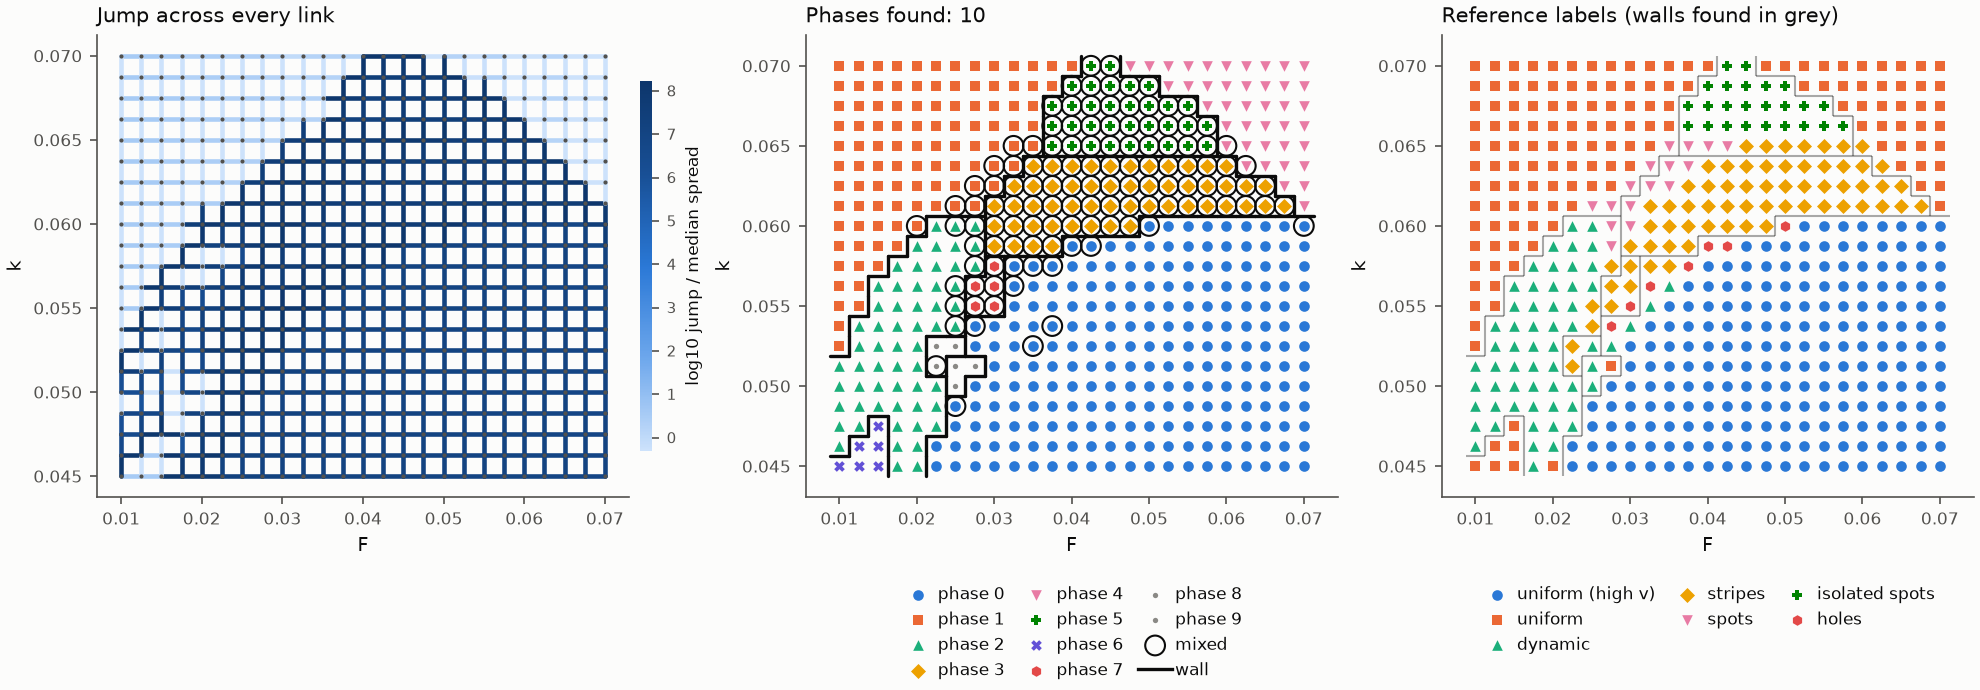
\includegraphics[width=\textwidth]{../examples/gray-scott/phase_map_hand.png}\\[2mm]
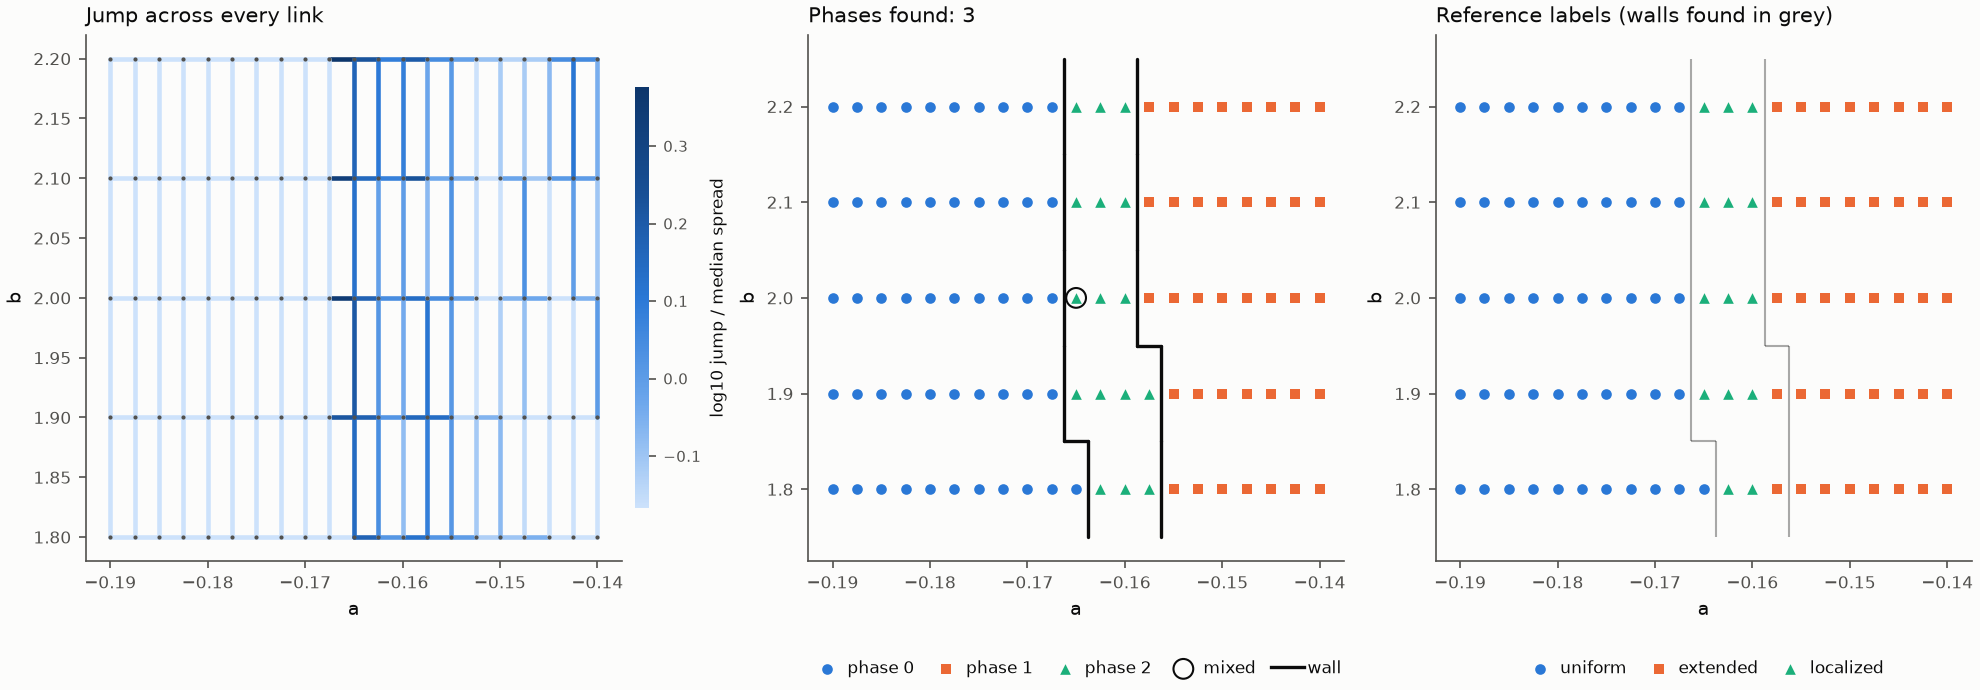
\includegraphics[width=\textwidth]{../examples/sh-localized/phase_map_hand.png}
\caption{Walls on the hand-made description. Top: Gray-Scott, $F$ from 0.010 to 0.070 and $k$ from
0.045 to 0.070 (steps 0.0025 and 0.00125), 4 runs per point to $t=40\,000$. Bottom: localised
Swift-Hohenberg, $a=\varepsilon/b^2$ from $-0.19$ to $-0.14$ and $b$ from 1.8 to 2.2, 4 runs per
point to $t=15\,000$. Left: jump across each link relative to the median spread; middle: phases
found (circles: mixed points); right: reference labels with the walls found in grey.}
\label{fig:examples}
\end{figure}

%======================================================================
\section{Choices}\label{sec:choices}
%======================================================================

Every threshold that is not imposed by the mathematics is a named constant with a comment
in the code saying it is a choice.

\begin{table}[H]
\centering\small
\begin{tabular}{@{}>{\raggedright}p{4.2cm}>{\raggedright}p{1.8cm}>{\raggedright\arraybackslash}p{8.0cm}@{}}
\toprule
Constant (file) & Value & Role and reason \\
\midrule
\code{FLAT} (describe) & $10^{-6}$ & fluctuations below this: flat field, descriptors at fixed floor values \\
\code{SHELL_RATIO} (describe) & 1.2 & width ratio of successive $|\mathbf k|$ shells (log spacing, no empty shell) \\
\code{DECOR_FLOOR} (describe) & $10^{-3}$ & floor of $1-C$: round-off of a frozen pattern is not motion \\
\code{LEVELS} (describe) & $-1,0,1$ & levels $z$ of the domain counts, in standard deviations \\
\code{DECIMALS} (graph) & 9 & parameter values rounded to identify a point \\
\code{ALPHA} (walls) & $10^{-3}$ & Mann-Whitney threshold; strict because links are correlated \\
\code{RATIO} (walls) & 1.5 & minimum ratio of median crossing to inner $J_2$ \\
\code{MIN_PHASE} (walls) & 3 & smallest phase and smallest side of a cut, in points \\
\code{FLOOR_QUANTILE} (walls) & 0.1 & jumps below this quantile of the spreads count as no jump \\
\code{MAX_PER_NODE} (walls) & 200 & snapshots per point used at most (cost of distances) \\
\code{MIXED_K} (walls) & 6 & robust $z$ above which a point is mixed ($E$ is right-skewed) \\
\code{MIN_WEIGHT} (walls) & $10^{-8}$ & lower bound of link weights: strong walls keep the graph connected \\
\code{SEEDS} (toy) & 8 & runs per demo point (6 is the fewest that finds the hexagon-stripe wall) \\
\code{UNIFORM_STD}, \code{HEXAGON_SKEW} & $10^{-3}$, 0.4 & reference labels of the demo only \\
\code{TUKEY_ALPHA} (describe) & 0.5 & tapered share of the window of non-periodic frames (4 times less leakage than none) \\
\code{MIN_WAVELENGTHS} (io) & 3 & non-periodic frames: $S(k)$ only for wavelengths up to $L_c/3$ \\
\code{MAX_SHIFT_FRACTION} (frames) & 0.2 & default \code{max_shift}: a fifth of the box side \\
\code{CHANNELS}, \code{HIDDEN}, \code{OUT} (nn) & 32--256, 256, 64 & sizes of $f$ and $g$ (as in hfml Step 7) \\
\code{T} (nn) & 0.2 & temperature of the InfoNCE loss \\
\code{PCA_VARIANCE}, \code{K_MIXTURE}, \code{K_KMEANS} (baselines) & 0.95, 1--10, 2--10 & blind grouping, as in hfml \\
\code{HDBSCAN_SIZES}, \code{FOLDS}, \code{C_PROBE} (baselines) & 5--40, 5, 1 & HDBSCAN sizes; probe folds and penalty \\
\code{Settings} (nn) & 40 epochs, batch 128 & AdamW, $10^{-3}$, warm-up 3 epochs, cosine decay, 4 draws per run and epoch \\
\bottomrule
\end{tabular}
\caption{Named choices. Block weighting, median imputation and alternate-run halves are
choices too (documented in their docstrings).}
\end{table}

%======================================================================
\section{Tests}\label{sec:tests}
%======================================================================

\code{pytest} runs 129 tests in about a minute, all on small synthetic data with known
answers (no data from any laboratory is in the repository). On every push, the
continuous-integration workflow \srcref{.github/workflows/tests.yml} runs \code{ruff} and
\code{pytest}.

\begin{table}[H]
\centering\small
\begin{tabular}{@{}l>{\raggedright\arraybackslash}p{11.6cm}@{}}
\toprule
File & What is checked, against which known answer \\
\midrule
\code{test_fields.py} & vector rule against the gradient of a rotated scalar; nematic rule against a turned director; group relations of $D_4$; shapes \\
\code{test_io.py} & round trips with and without Julia layout; first key found; snapshot list sorted by time; TOML configuration and its errors \\
\code{test_describe.py} & shells cover the grid; $S(k)$ of one wave; exact moments; periodic domain counts; spots $m^2$ against stripes $m$; flat fields; flows; global order; dynamics; invariance of every descriptor under $D_4$ and shifts; tables and error list \\
\code{test_graph.py} & nodes merge rounding errors; links of a full grid, of a refined line, of one parameter; numbering of regions \\
\code{test_walls.py} & energy distance; halves; feature matrix; cut of a chain; no wall in noise (5 seeds) or a smooth drift; two and three phases with the exact walls; mixed point; count against \code{RATIO} \\
\code{test_toy.py} & states at six points; stripe amplitude $\sqrt{2\varepsilon/3}$; seeds differ; ensemble readable \\
\code{test_report.py} & wall segments at $a=5.5$; phase extents and summary; files written; one-parameter scans \\
\code{test_cli.py} & \code{describe}, \code{walls}, \code{demo --quick}; labels per point; exit status 0 \\
\code{test_nn.py} & augmentations against the field rules; shift invariance of a periodic encoder; loss at collapse and for perfect pairs; a short training separates stripes from spots; saving and loading; \code{learn} and \code{describe --encoder} (skipped without PyTorch) \\
\code{test_baselines.py} & separated clouds found by the mixture, k-means and HDBSCAN; groups in two places counted as two pieces; probe on real and random labels; no ARI without placed points (skipped without scikit-learn) \\
\code{test_frames.py} & crops, coarsening and their errors; $S(k)$ of crops against the exact one; finite against spectral derivatives; windowed moving correlation; rotation and mirror invariance; $\Delta x$ against $\Delta x/2$; mixed grids \\
\bottomrule
\end{tabular}
\end{table}

%======================================================================
\section{Limitations and next steps}\label{sec:limits}
%======================================================================

\begin{itemize}[leftmargin=1.2em]
\item \textbf{Only what the descriptors see.} Two states with the same descriptors form one
  phase. The descriptor table can be replaced by any other description (for example one
  learned by a self-supervised network) without changing the rest.
\item \textbf{Only the states the runs reach.} Hidden bistability (Sec.~\ref{sec:demo}) needs
  runs from several kinds of initial conditions.
\item \textbf{Power against bias.} The split into halves removes the selection bias but needs
  enough runs per point (6 to 8 in the demo for a weak wall).
\item \textbf{Correlated links.} $p$ is a score; its threshold was set on synthetic tests and
  the demo, not derived.
\item \textbf{Non-periodic frames.} The moving correlation sees displacements up to
  \code{max_shift} only; $S(k)$ is measured for wavelengths up to $L_c/3$ only.
\item \textbf{Grids.} Links join neighbours along one parameter at a time; scattered (non-grid)
  samples would need another graph, for example nearest neighbours.
\item \textbf{Learned description.} On the demo it carries the state but without a jump at the
  hexagon-stripe boundary (Sec.~\ref{sec:comparison}), so the walls method finds two phases of three.
\item \textbf{One state per point.} Where many points have runs that end in different states
  (FitzHugh-Nagumo; plane waves and spirals in Barkley; Sec.~\ref{sec:examples-results}), the spread of a point is as large as the
  jumps and no wall is found. A description of each point as a mixture of states is needed there.
\item \textbf{Odd fields.} A symmetry $u\to-u$ of the equations is not used by the description
  (the mean and the skewness change sign); a field rule for odd fields would make them even.
\item \textbf{Next.} A training objective for the learned description that rewards differences
  between phases; why the learned block dominates the combined table; a stopping rule for the
  tree that does not over-split (Gray-Scott) and works with one run per point.
\end{itemize}

%======================================================================
\section{Map of the code}\label{sec:map}
%======================================================================

\begin{table}[H]
\centering\small
\begin{tabular}{@{}l>{\raggedright}p{7.0cm}l@{}}
\toprule
File & Content & Section \\
\midrule
\srcref{src/phasewall/fields.py} & field kinds, symmetries of the box & \ref{sec:fields} \\
\srcref{src/phasewall/io.py} & TOML configuration, reading and writing snapshots & \ref{sec:fields} \\
\srcref{src/phasewall/describe.py} & descriptors of snapshots and ensembles & \ref{sec:describe} \\
\srcref{src/phasewall/frames.py} & crops, coarsening, non-periodic frames & \ref{sec:frames} \\
\srcref{src/phasewall/nn/} & learned description: data, model, loss, training & \ref{sec:learned} \\
\srcref{src/phasewall/baselines.py} & blind grouping and logistic probe, for comparison & \ref{sec:methods} \\
\srcref{src/phasewall/trees.py} & unsupervised threshold tree & \ref{sec:tree} \\
\srcref{src/phasewall/graph.py} & nodes and links of the scan, regions & \ref{sec:compare} \\
\srcref{src/phasewall/walls.py} & features, distances, cuts, tests, mixed points & \ref{sec:compare}--\ref{sec:mixed} \\
\srcref{src/phasewall/toy.py} & Swift-Hohenberg demo & \ref{sec:demo} \\
\srcref{src/phasewall/gray_scott.py} & Gray-Scott example: simulation, reference labels & \ref{sec:examples} \\
\srcref{src/phasewall/fitzhugh_nagumo.py} & FitzHugh-Nagumo example & \ref{sec:examples} \\
\srcref{src/phasewall/barkley.py} & Barkley example, spiral tips & \ref{sec:examples} \\
\srcref{src/phasewall/sh_localized.py} & localised Swift-Hohenberg example & \ref{sec:examples} \\
\srcref{src/phasewall/examples.py} & registry of the examples & \ref{sec:examples} \\
\srcref{src/phasewall/pipeline.py} & whole analysis in one call, cached steps (used by the interface and the scripts) & \ref{sec:examples} \\
\srcref{src/phasewall/scores.py} & agreement, ARI, pieces on the grid & \ref{sec:methods} \\
\srcref{src/phasewall/report.py} & summary, tables, figures & \ref{sec:demo} \\
\srcref{src/phasewall/cli.py} & command-line tool & \ref{sec:overview} \\
\srcref{scripts/doc_figures.py} & data figures of this document & all \\
\srcref{scripts/compare_describers.py} & descriptions and methods compared on the demo & \ref{sec:comparison}, \ref{sec:methods} \\
\srcref{scripts/run_examples.py} & all examples: steady-state check, descriptions, methods & \ref{sec:examples-results} \\
\srcref{scripts/tree_examples.py} & the tree on all examples & \ref{sec:examples-results} \\
\srcref{tests/} & 129 tests & \ref{sec:tests} \\
\bottomrule
\end{tabular}
\end{table}

\paragraph{References.}
J.~Swift and P.~C.~Hohenberg, Phys.\ Rev.\ A \textbf{15}, 319 (1977).
M.~C.~Cross and P.~C.~Hohenberg, Rev.\ Mod.\ Phys.\ \textbf{65}, 851 (1993).
R.~Hoyle, \emph{Pattern Formation} (Cambridge University Press, 2006), hexagons and stripes.
G.~J.~Sz\'ekely and M.~L.~Rizzo, J.\ Stat.\ Plann.\ Inference \textbf{143}, 1249 (2013), energy statistics.
J.~Shi and J.~Malik, IEEE Trans.\ PAMI \textbf{22}, 888 (2000), normalised cuts.
J.~E.~Pearson, Science \textbf{261}, 189 (1993), Gray-Scott patterns.
A.~Hagberg and E.~Meron, Phys.\ Rev.\ Lett.\ \textbf{72}, 2494 (1994), FitzHugh-Nagumo fronts.
D.~Barkley, Physica D \textbf{49}, 61 (1991), excitable media.
J.~Burke and E.~Knobloch, Phys.\ Rev.\ E \textbf{73}, 056211 (2006), localised states.
U.~von Luxburg, Stat.\ Comput.\ \textbf{17}, 395 (2007), spectral clustering.
H.~B.~Mann and D.~R.~Whitney, Ann.\ Math.\ Stat.\ \textbf{18}, 50 (1947).

\end{document}
